\documentclass[9pt,aspectratio=169]{beamer}
\usetheme[progressbar=frametitle,numbering=fraction]{metropolis}
\usepackage{amsmath,amssymb,amsthm,mathtools,booktabs,bm}
\usepackage{graphicx}
\graphicspath{{../figures/}}

\definecolor{accent}{HTML}{2A78D6}
\definecolor{warn}{HTML}{C0392B}
\setbeamercolor{alerted text}{fg=warn}
\setbeamercolor{block title}{bg=accent!15,fg=black}
\setbeamercolor{block body}{bg=accent!5}
\setbeamertemplate{theorems}[numbered]
\theoremstyle{plain}
\newtheorem{proposition}{Proposition}
\newtheorem{remarkx}{Remark}

\newcommand{\R}{\mathbb{R}}
\newcommand{\x}{\mathbf{x}}
\newcommand{\cc}{\mathbf{c}}
\newcommand{\pp}{\mathbf{p}}
\newcommand{\w}{\mathbf{w}}
\newcommand{\q}{\mathbf{q}}
\newcommand{\h}{\mathbf{h}}
\newcommand{\Ot}{\tilde O}
\newcommand{\ysum}{\mathbin{\dot{+}}}
\newcommand{\sat}{\operatorname{sat}}
\newcommand{\artanh}{\operatorname{artanh}}
\DeclareMathOperator{\core}{core}

\title{A Fuzzy Set--Based Methodology for Autonomous Navigation}
\subtitle{Implementation and mathematical analysis}
\institute{Paper: E.\,A.~Rastkhiz, H.~Schwartz, I.~Lambadaris, \emph{Fuzzy Sets and Systems} 518 (2025) 109485}
\author{Fuzzy Logic --- course project}
\date{}

\begin{document}

\maketitle

% ---------------------------------------------------------------------------
\begin{frame}{The problem and the idea in one slide}
\begin{columns}[T]
\column{0.52\textwidth}
\textbf{Given}
\begin{itemize}
  \item a global path, as crisp waypoints $\w_1,\dots,\w_M$;
  \item local objects $O_i$ (position $\cc_i$, velocity $v_i$), perceived \emph{imprecisely}.
\end{itemize}
\textbf{Want} a motion that stays close to the path \emph{and} avoids the objects.

\medskip
\textbf{Idea of the paper}
\begin{enumerate}
  \item Model obstacles \emph{and} path as fuzzy subsets of $\R^2$.
  \item Merge them with a Yager t-conorm into one fuzzy set $E$.
  \item Drive along a level curve $\{\mu_E=\mu_{th}\}$; lower the level near obstacles.
\end{enumerate}
\column{0.46\textwidth}
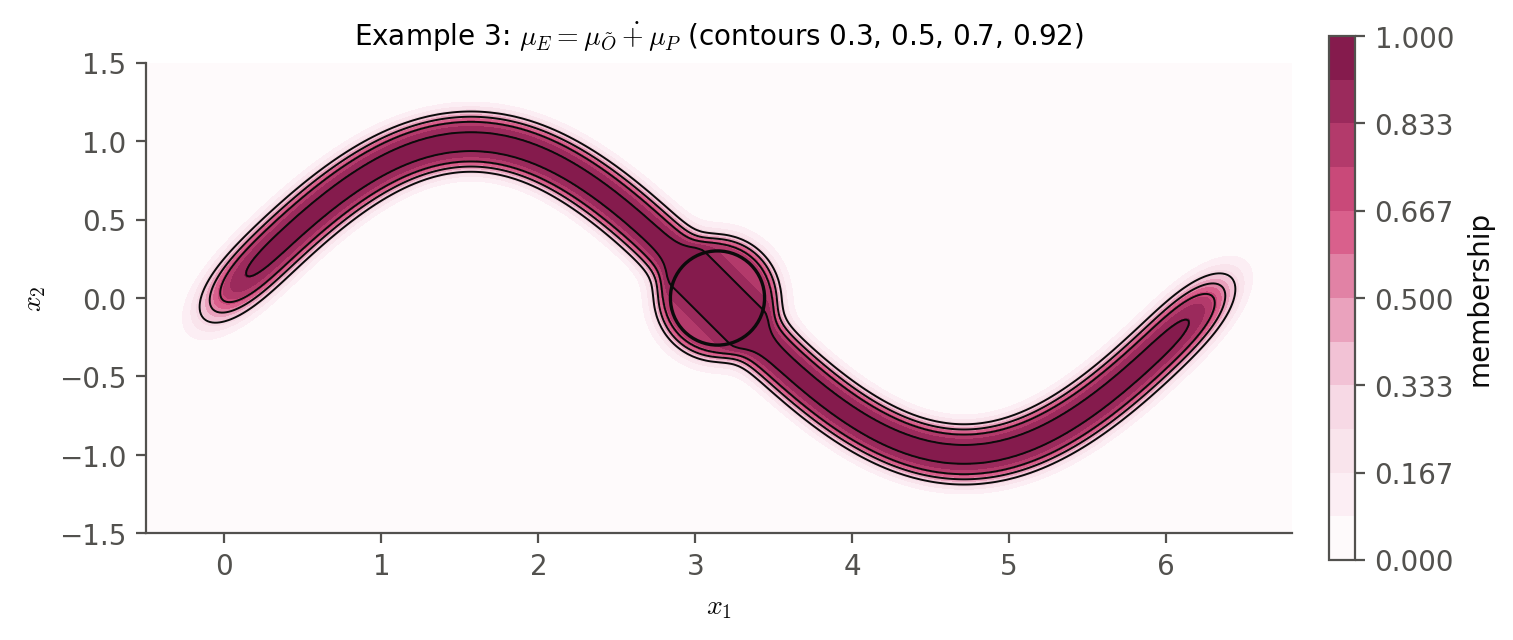
\includegraphics[width=\linewidth]{f05_example3_env.png}

\small Contours of $\mu_E$ bend around the obstacle, so they are themselves candidate paths.
\end{columns}
\end{frame}

\begin{frame}{Outline}
\begin{enumerate}
  \item Fuzzy preliminaries: $\alpha$-cuts, convexity, Yager t-conorms
  \item The fuzzy environment model: obstacles, path, environment
  \item Path planning as an optimisation problem on $\mu_E$
  \item \alert{Our analysis}: a Lyapunov argument, the orientation lemma, and a feasibility condition (Poisson summation)
  \item Simulations (Python re-implementation) and critical assessment
\end{enumerate}
\vfill
\small Everything marked \emph{Our analysis} goes beyond the paper; everything else follows it, eq.\ numbers $(\cdot)$ refer to the paper.
\end{frame}

% ===========================================================================
\section{Fuzzy preliminaries}
% ===========================================================================
\begin{frame}{Fuzzy sets, $\alpha$-cuts, convexity}
A fuzzy set $A$ on $X=\R^2$ is a map $\mu_A : X\to[0,1]$. For $\alpha\in(0,1]$:
\[
  A_\alpha=\{\x\in X:\ \mu_A(\x)\ge\alpha\}\quad(\alpha\text{-cut}),\qquad
  \core A = A_1,\qquad A\text{ normal}\iff \sup\mu_A = 1 .
\]
\begin{block}{Definition (Def.~2 of the paper; Zadeh 1965)}
A normal fuzzy set is \emph{convex} iff every $A_\alpha$ is convex, equivalently iff $\mu_A$ is quasi-concave:
\[
  \mu_A(\lambda\x+(1-\lambda)\mathbf y)\ \ge\ \min\{\mu_A(\x),\mu_A(\mathbf y)\}\qquad\forall\,\lambda\in[0,1].
\]
\end{block}
\begin{itemize}
  \item Def.~1 of the paper calls the \emph{core} ``the central point of the $1$-cut''; for the sets used here the $1$-cut is a single point, see Prop.~\ref{prop:bmf}.
  \item Convexity is preserved under affine maps $\x\mapsto\Lambda^{-1}(\x-\cc)$, since $\alpha$-cuts map to affine images of convex sets.
  \item Convexity is \alert{not} preserved under union: the environment $E$ is not convex, only its building blocks are.
\end{itemize}
\end{frame}

\begin{frame}{t-conorms and Yager's class}
A \textbf{t-conorm} $S:[0,1]^2\to[0,1]$ is commutative, associative, monotone and has neutral element $0$: $S(a,0)=a$. It models the union: $\mu_{A\cup B}=S(\mu_A,\mu_B)$.
\begin{block}{Definition 3 (Yager 1980)}
For $p\in(0,\infty]$:\qquad
$\displaystyle S_p(a,b)=a\ysum b=\min\!\Big(1,(a^p+b^p)^{1/p}\Big)=\sat\big(\|(a,b)\|_p\big).$
\end{block}
\begin{proposition}[ordering and limits]\label{prop:order}
For fixed $a,b$, $p\mapsto S_p(a,b)$ is non-increasing, and
\[
\underbrace{\max(a,b)}_{p=\infty}\ \le\ S_p(a,b)\ \le\ \underbrace{\min(1,a+b)}_{p=1}\ \le\ \underbrace{S_D(a,b)}_{p\to0^+}
\]
where $S_D$ is the drastic sum ($=a$ if $b=0$, $=b$ if $a=0$, else $1$).
\end{proposition}
\emph{Proof.} $\|\cdot\|_p$ is non-increasing in $p$ and $\|\cdot\|_p\to\|\cdot\|_\infty=\max$; for $a,b>0$, $(a^p+b^p)^{1/p}\ge 2^{1/p}\min(a,b)\to\infty$ as $p\to0^+$. \qed

\small\alert{Remark.} The paper restricts to $p\ge1$, where the most conservative member is the \emph{bounded sum} ($p=1$), not the drastic sum.
\end{frame}

\begin{frame}{The Yager union, seen graphically}
\centering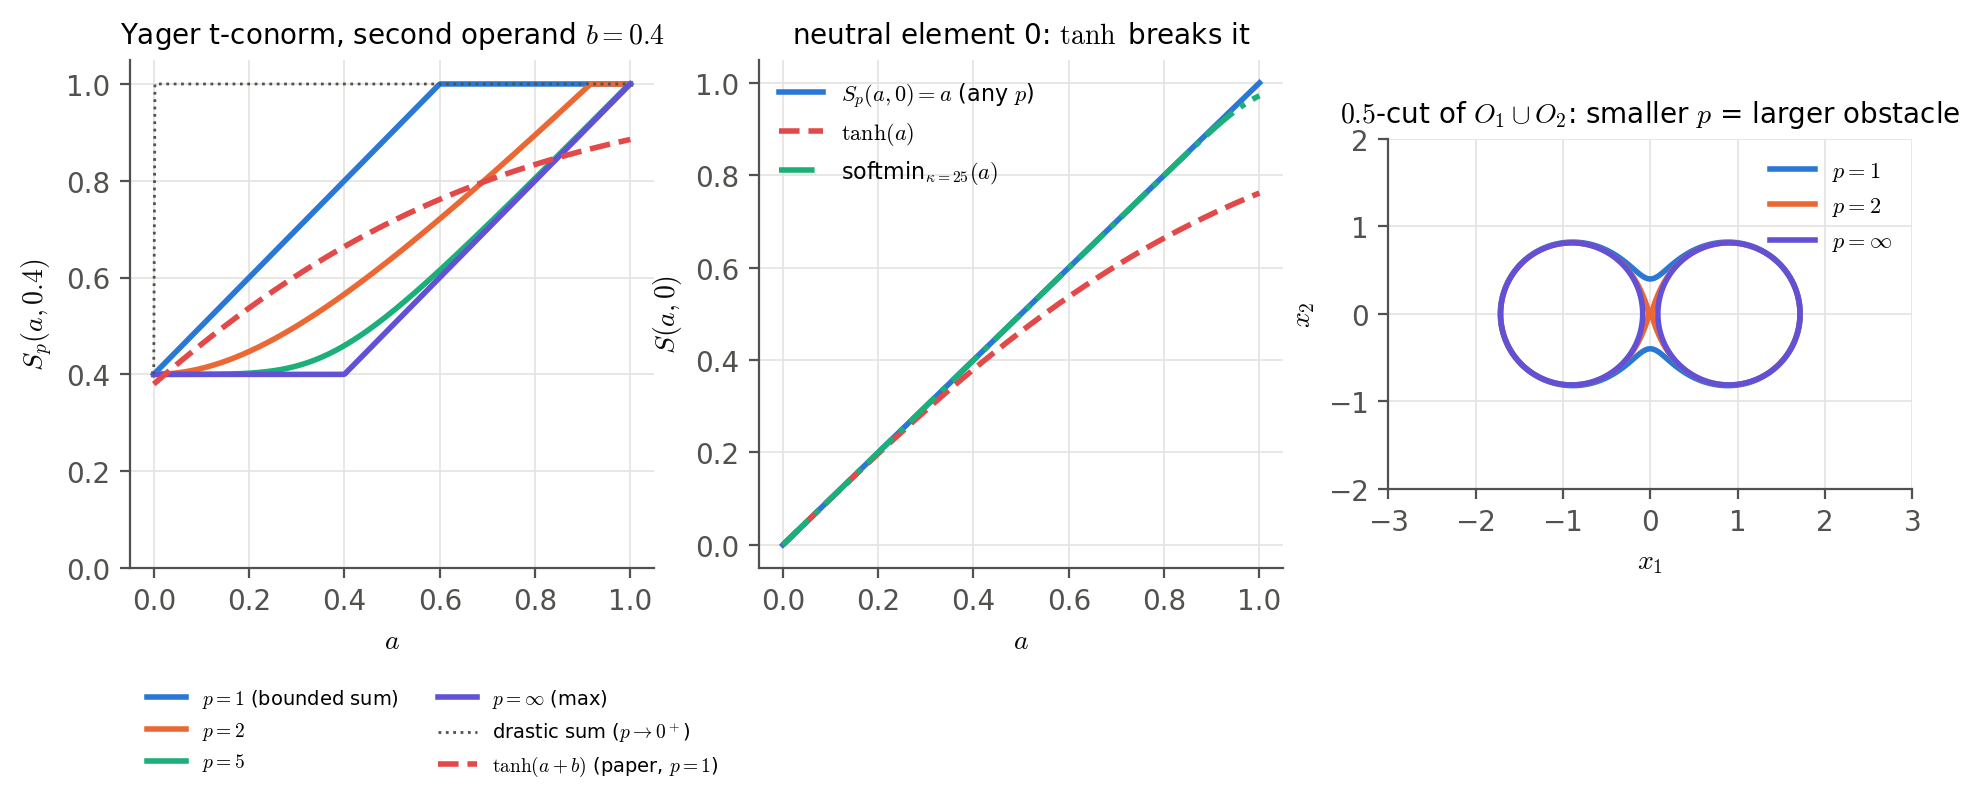
\includegraphics[width=\linewidth]{f02_yager.png}

\small Left: $S_p(a,0.4)$ for several $p$, plus the paper's smoothed $\tanh(a+b)$. Middle: the boundary law $S(a,0)=a$ and how $\tanh$ violates it. Right: the $0.5$-cut of a union of two discs; smaller $p$ gives a larger (more conservative) obstacle.
\end{frame}

\begin{frame}{Remark 1: the $m$-ary Yager t-conorm}
\begin{proposition}[Remark 1 of the paper]
For $a_1,\dots,a_m\in[0,1]$:\qquad
$a_1\ysum a_2\ysum\cdots\ysum a_m=\min\!\Big(1,\big(\textstyle\sum_{i=1}^m a_i^p\big)^{1/p}\Big)=\sat\big(\|\mathbf a\|_p\big).$
\end{proposition}
\emph{Proof} (induction on $m$; $m=2$ is the definition). Let $n=\|(a_1,\dots,a_{m-1})\|_p$ and assume the claim for $m-1$.
\begin{itemize}
  \item If $n<1$: the left-hand side is $\min\!\big(1,(n^p+a_m^p)^{1/p}\big)=\min(1,\|\mathbf a\|_p)$.
  \item If $n\ge1$: the first $m-1$ terms give $1$, and $1\ysum a_m=\min(1,(1+a_m^p)^{1/p})=1$. Also $\|\mathbf a\|_p\ge n\ge1$, so the right-hand side is $1$ too. \qed
\end{itemize}
\textbf{Consequences}
\begin{itemize}
  \item Associativity of $S_p$ follows, because the right-hand side is symmetric in all $a_i$.
  \item The union of $N$ atoms costs one $p$-norm, $\mathcal O(N)$. With $\sat$ smoothed, $\mu_E$ becomes a closed-form, differentiable function of $\x$.
\end{itemize}
\end{frame}

\begin{frame}{Smoothing the saturation: what is lost}
The planner needs $\nabla\mu_E$, so the paper replaces $\sat(u)=\min(1,u)$ by $\tanh(u)$:
\[
  \tilde S(\mathbf a)=\tanh\big(\|\mathbf a\|_p\big).
\]
\begin{proposition}[Our analysis]\label{prop:tanh}
$\tilde S$ is symmetric, monotone and $C^\infty$ on $(0,1]^m$, but it is \alert{not a t-conorm}:
\begin{enumerate}
  \item no neutral element: $\tilde S(a,0)=\tanh a<a$ for $a>0$ (e.g.\ $\tilde S(1,0)=0.762$);
  \item not associative: $\tilde S(\tilde S(a,b),c)\ne\tilde S(a,b,c)$ in general, so $E=\Ot\cup P$ depends on how the union is bracketed;
  \item $\tilde S(\mathbf a)<1$ for all finite inputs, so the union is never normal.
\end{enumerate}
\end{proposition}
\textbf{A range-preserving alternative} (used in our runs) is the softplus smooth minimum
\[
\sat_\kappa(u)=u-\tfrac1\kappa\log\!\big(1+e^{\kappa(u-1)}\big)+c_\kappa,\qquad
0\le \min(1,u)-\sat_\kappa(u)\le \tfrac{\ln2}{\kappa}+|c_\kappa| ,
\]
which converges uniformly to $\sat$ as $\kappa\to\infty$; we take $\kappa=25$. \emph{Proof:} $0\le\log(1+e^z)-\max(0,z)\le\ln2$.
\end{frame}

% ===========================================================================
\section{The fuzzy environment model}
% ===========================================================================
\begin{frame}{Obstacle base membership function}
\begin{columns}[T]
\column{0.5\textwidth}
\[
  \mu(\chi)=\tanh\!\big((\chi^T\chi)^{-b}\big),\qquad b\ge1 \tag{6}
\]
\begin{proposition}[Our analysis]\label{prop:bmf}
Let $\rho=\|\chi\|_2$.
\begin{enumerate}
  \item $\mu$ is radial, strictly decreasing in $\rho$, with $\mu\to1$ as $\rho\to0$. So the core is $\{0\}$ and $\mu$ is convex.
  \item $\mu_\alpha=\{\rho\le(\artanh\alpha)^{-1/(2b)}\}$.
  \item For every $b$, the $\tanh(1)$-cut is exactly the unit disc.
  \item As $b\to\infty$, $\mu\to\mathbf 1_{\{\rho<1\}}$ (and $\tanh 1$ on $\rho=1$).
\end{enumerate}
\end{proposition}
\vspace{-1ex}
\small (3) and (4) make precise the paper's phrase ``the core is the unit circle''.
\column{0.48\textwidth}
\vspace{-1ex}
\[
\nabla_\chi\mu=-2b\,\operatorname{sech}^2\!\big(s^{-b}\big)\,s^{-b-1}\chi,\quad s=\chi^T\chi
\]
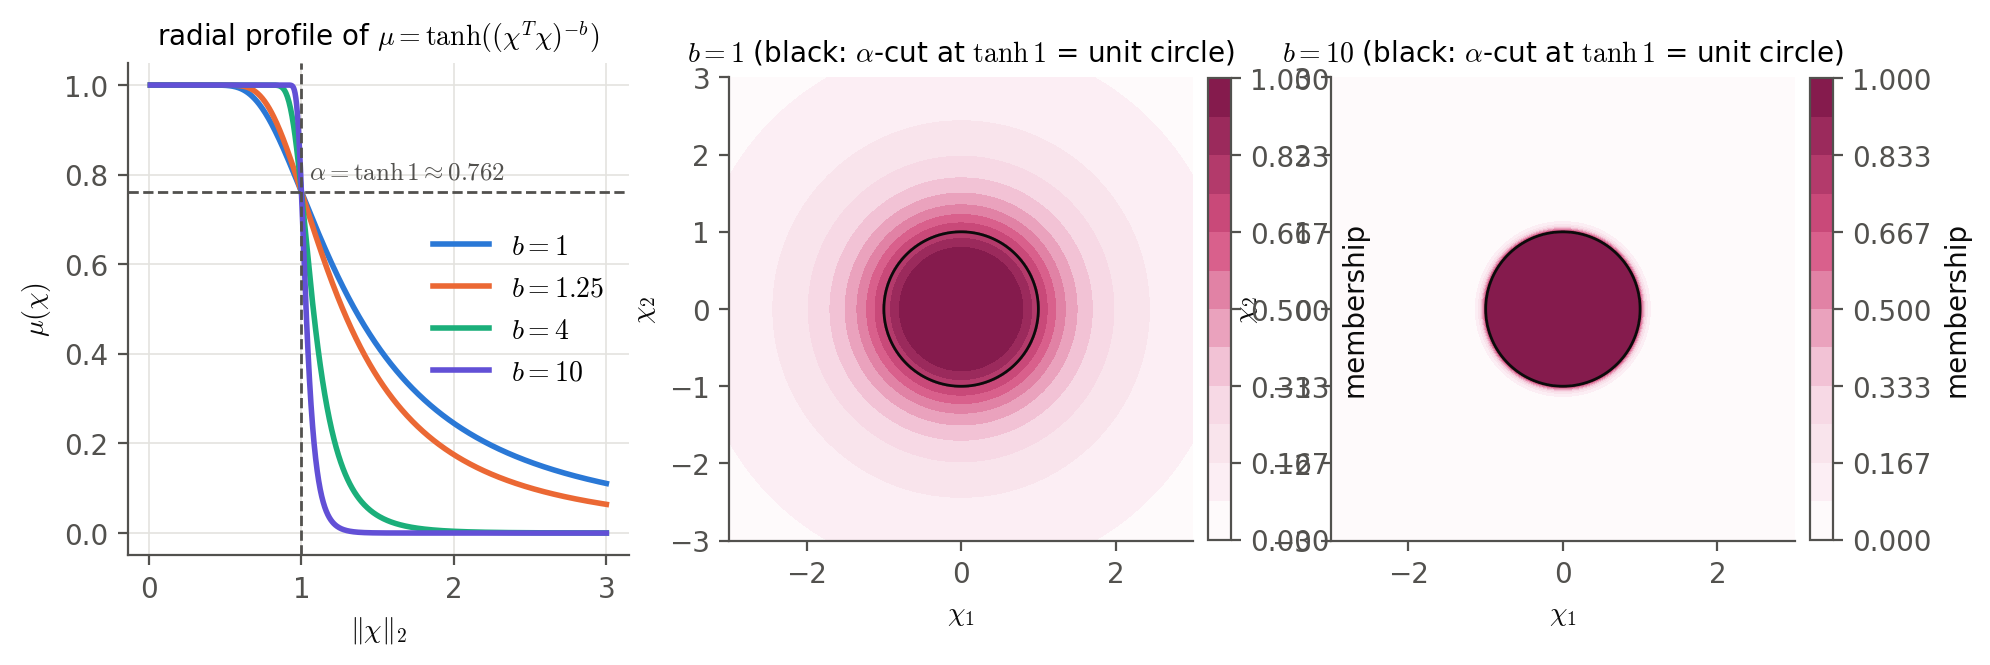
\includegraphics[width=\linewidth]{f01_bell_bmf.png}
\end{columns}
\end{frame}

\begin{frame}{Atomic obstacles and velocity inflation}
Each object is covered by atoms. Atom $i$ is a transformed copy of the BMF:
\[
  \mu_{\Ot_i}(\x)=\mu\big(\Lambda_i^{-1}(\x-\cc_i)\big),\qquad
  \Lambda_i=(\lambda_i+r_i)I_2+[\q_i,\q_i^\perp]\begin{bmatrix}\delta\|v_i\|&0\\0&0\end{bmatrix}[\q_i,\q_i^\perp]^T \tag{2--3}
\]
\begin{itemize}
  \item $\Lambda_i$ is symmetric positive definite, with spectral decomposition
  $\Lambda_i=(\lambda_i+r_i+\delta\|v_i\|)\,\q_i\q_i^T+(\lambda_i+r_i)\,\q_i^\perp\q_i^{\perp T}$.
  \item $\alpha$-cuts are ellipses $\{(\x-\cc_i)^T\Lambda_i^{-2}(\x-\cc_i)\le\rho_\alpha^2\}$ with semi-axes $\rho_\alpha(\lambda_i+r_i+\delta\|v_i\|)$ along $v_i$ and $\rho_\alpha(\lambda_i+r_i)$ across it.
  \item Chain rule: $\nabla_\x\mu_{\Ot_i}=\Lambda_i^{-1}\nabla_\chi\mu$, since $\Lambda_i=\Lambda_i^T$.
  \item \small The inflation is symmetric, \emph{behind} the object as well as ahead of it; an asymmetric $\Lambda_i$ would be a natural refinement.
\end{itemize}
\centering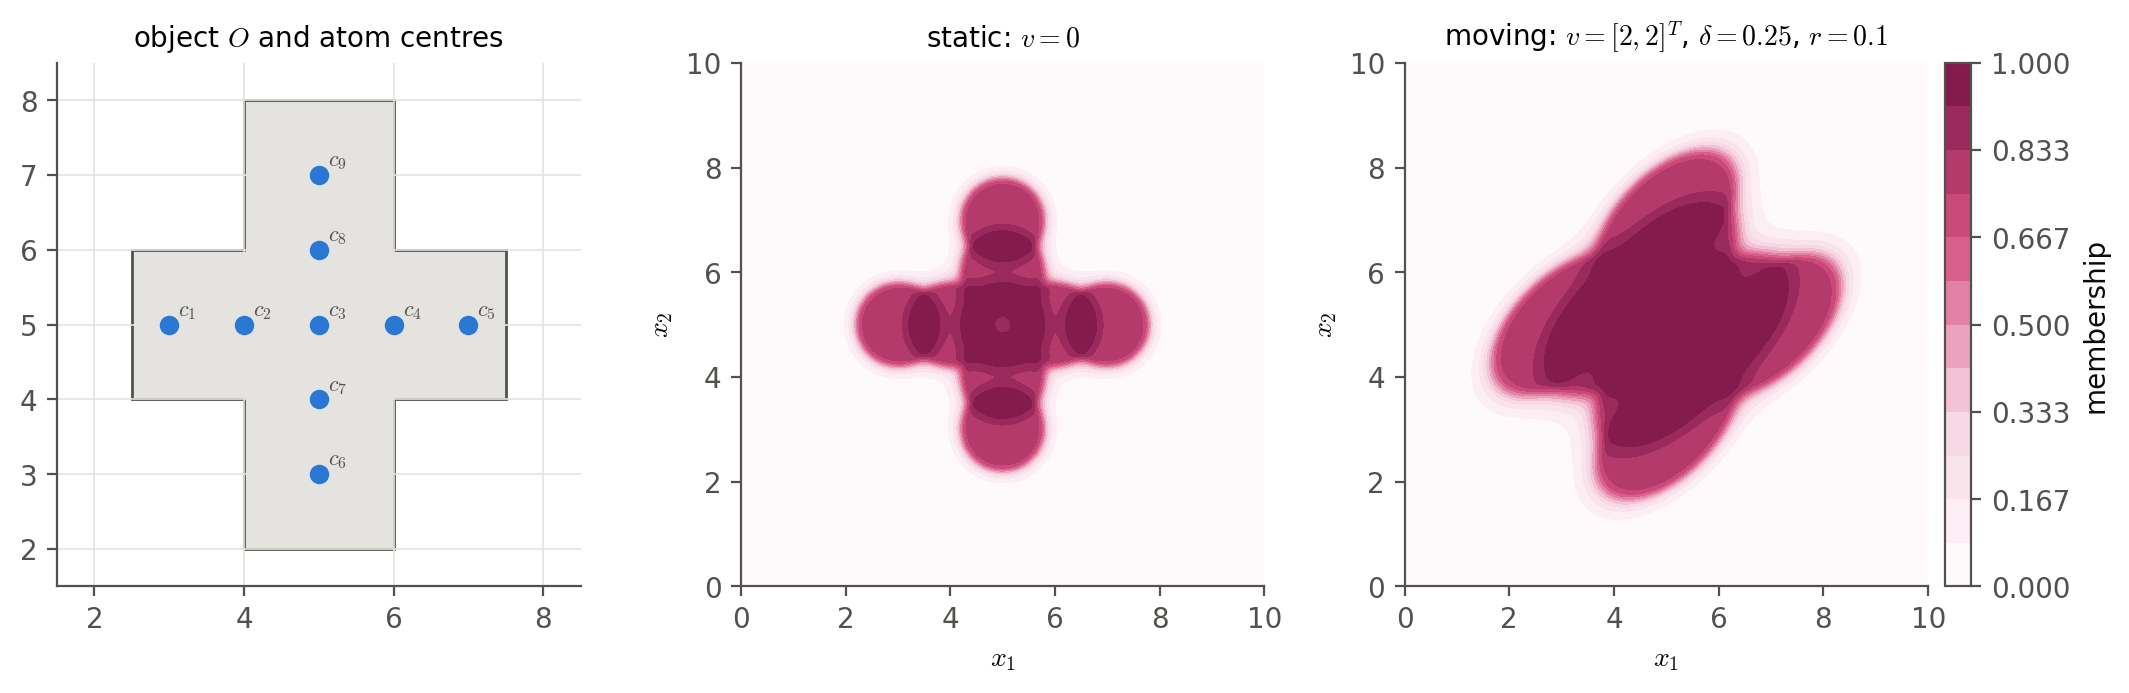
\includegraphics[width=0.52\linewidth]{f03_example1_obstacle.png}
\end{frame}

\begin{frame}{Collective obstacle region}
\[
  \Ot=\bigcup_{i=1}^N\Ot_i,\qquad \mu_{\Ot}(\x)=\mu_{\Ot_1}(\x)\ysum\cdots\ysum\mu_{\Ot_N}(\x)=\sat\Big(\big(\textstyle\sum_i\mu_{\Ot_i}(\x)^p\big)^{1/p}\Big)\tag{4--5}
\]
\begin{itemize}
  \item Since $S_p\ge\max$, we have $\Ot_\alpha\supseteq\bigcup_i(\Ot_i)_\alpha$: the union never \emph{shrinks} an obstacle. Equality holds for $p=\infty$.
  \item With $p=1$ (used in all simulations of the paper), overlapping atoms reinforce each other. Gaps between neighbouring atoms are filled, so a chain of discs behaves like a wall.
  \item Gradient of the smoothed union (exact, used by our code):
  \[
    \nabla\mu_{\Ot}=\sat'(n)\sum_i\Big(\tfrac{\mu_{\Ot_i}}{n}\Big)^{p-1}\nabla\mu_{\Ot_i},\qquad n=\big\|(\mu_{\Ot_i})_i\big\|_p .
  \]
\end{itemize}
\small Checked against central differences at 200 random points for all $p\in\{1,2,5\}$ and all saturations: max.\ relative error $2\times10^{-9}$.
\end{frame}

\begin{frame}{The fuzzy path: Gaussian fuzzy waypoints}
\[
\xi(\chi)=e^{-\frac12\chi^T\chi},\qquad
\mu_{W_j}(\x)=\xi\big(\Gamma_j^{-1}(\x-\pp_j)\big)=\exp\!\Big(-\tfrac12(\x-\pp_j)^T\Gamma_j^{-2}(\x-\pp_j)\Big)\tag{8--9}
\]
\[
\pp_j=\tfrac12(\w_j+\w_{j+1}),\qquad \Gamma_j=H_j\begin{bmatrix}\gamma\|\w_{j+1}-\w_j\|&0\\0&\sigma_j\end{bmatrix}H_j^T,\quad H_j=[\h_j,\h_j^\perp].\tag{10}
\]
\begin{itemize}
  \item The core is the singleton $\{\pp_j\}$, and $\mu_{W_j}$ is convex: a crisp waypoint generalised to a fuzzy one.
  \item $\Gamma_j$ is a \emph{standard deviation} matrix: std.\ $\gamma\|\Delta\w\|$ along the segment and $\sigma_j$ across it.
  \item \small\alert{Notational remark:} the paper prints $H_j^T D H_j$. With $\h_j$ as columns of $H_j$, the matrix with eigenvector $\h_j$ is $H_jDH_j^T$, as in (3). We implement $H_jDH_j^T$.
\end{itemize}
\[
 P=\bigcup_j W_j,\qquad \mu_P=\mu_{W_1}\ysum\cdots\ysum\mu_{W_{M-1}}\tag{11--12}
\]
\end{frame}

\begin{frame}{Fuzzy path (Example 2) and environment (Example 3)}
\begin{columns}[T]
\column{0.5\textwidth}
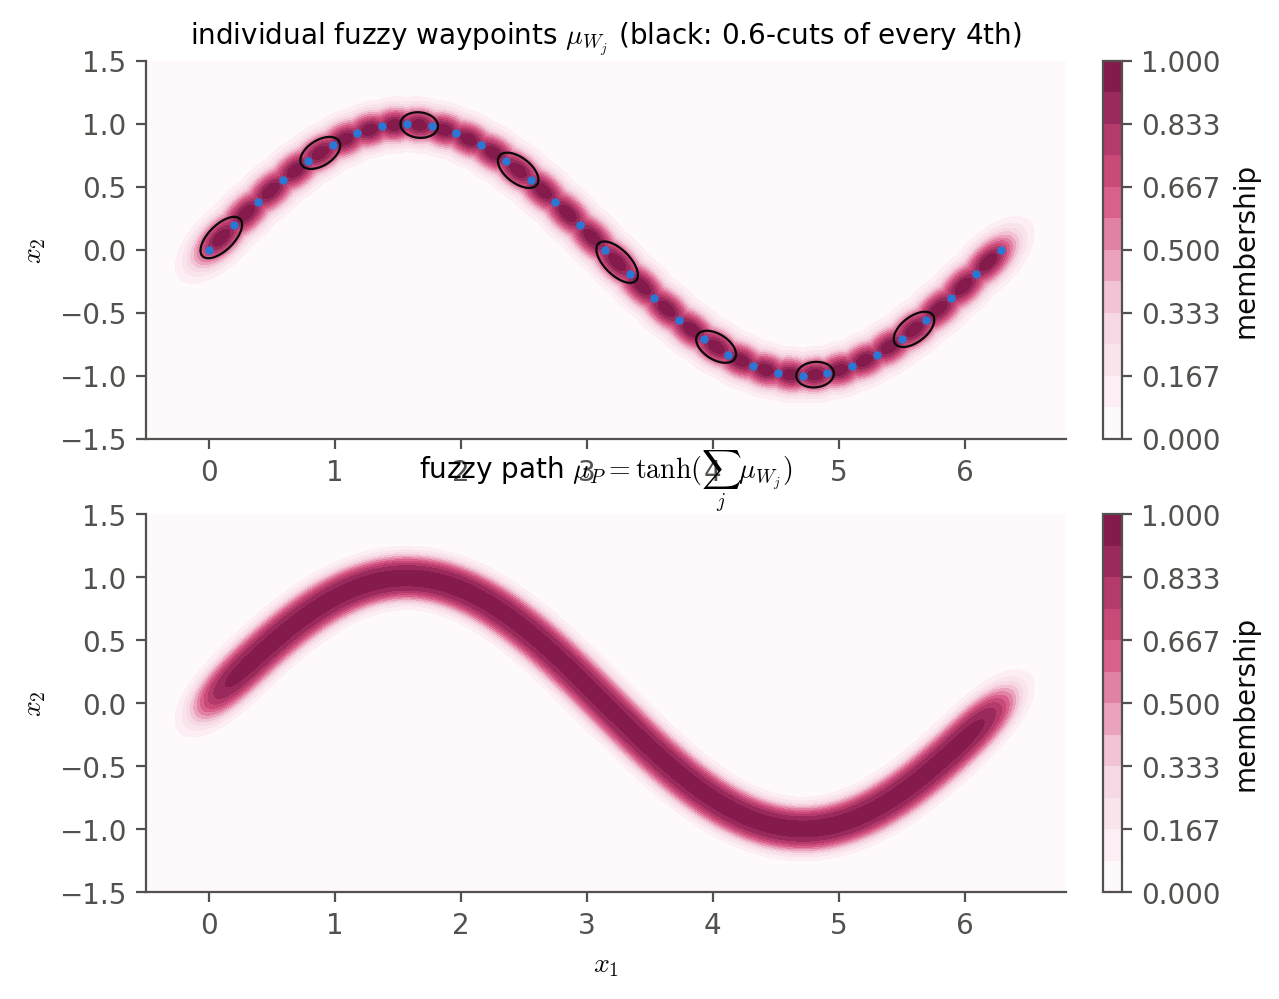
\includegraphics[width=\linewidth]{f04_example2_path.png}
\column{0.5\textwidth}
\[
E^k=\Ot^k\cup P,\qquad \mu_{E^k}=\mu_{\Ot^k}\ysum\mu_P\tag{15--16}
\]
\begin{itemize}
  \item The path is a ``virtual obstacle'' whose membership is \emph{desirable}.
  \item A dynamic scene is a sequence of static episodes $E^k$, one per sampling interval $t_s$.
  \item Implementation choice: because $\tilde S$ is not associative, we evaluate $E$ as one $m$-ary union of all atoms (Remark~1).
\end{itemize}
\centering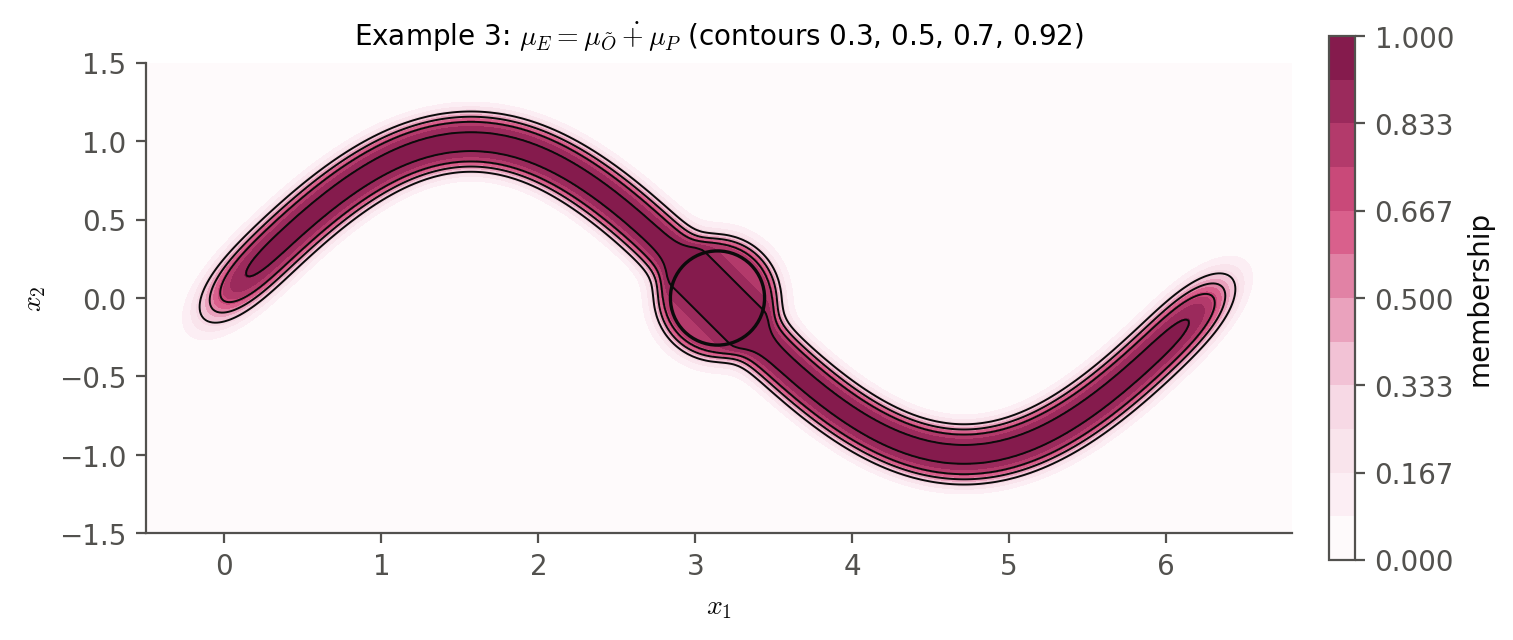
\includegraphics[width=0.8\linewidth]{f05_example3_env.png}
\end{columns}
\end{frame}

% ===========================================================================
\section{Path planning on the fuzzy environment}
% ===========================================================================
\begin{frame}{Level curves as a family of paths; adaptive level and speed}
The level curves $C_h=\{\x:\mu_{E^k}(\x)=h\}$, $h\in(0,1]$, are candidate paths: high $h$ means close to the global path, low $h$ means far from obstacles.
\[
\mu_{th}=\alpha\big(1-\mu_{\Ot^k}(\x_k)\big)^{d_o}\quad(17)\qquad\qquad
v_{max}=v_m\big(1-\mu_{\Ot^k}(\x_k)\big)^{d_v}\quad(18)
\]
\textbf{Tuning by two extreme cases} (solving for the exponent with logarithms):
\[
\alpha=0.99,\ \mu_{\Ot}=0.99,\ \mu_{th}=0.01\ \Rightarrow\ d_o=\frac{\ln(0.01/0.99)}{\ln 0.01}=0.9978,
\qquad
\frac{v_{max}}{v_m}=\frac{1}{10}\ \Rightarrow\ d_v=\frac{\ln0.1}{\ln0.01}=0.5 .
\]
\centering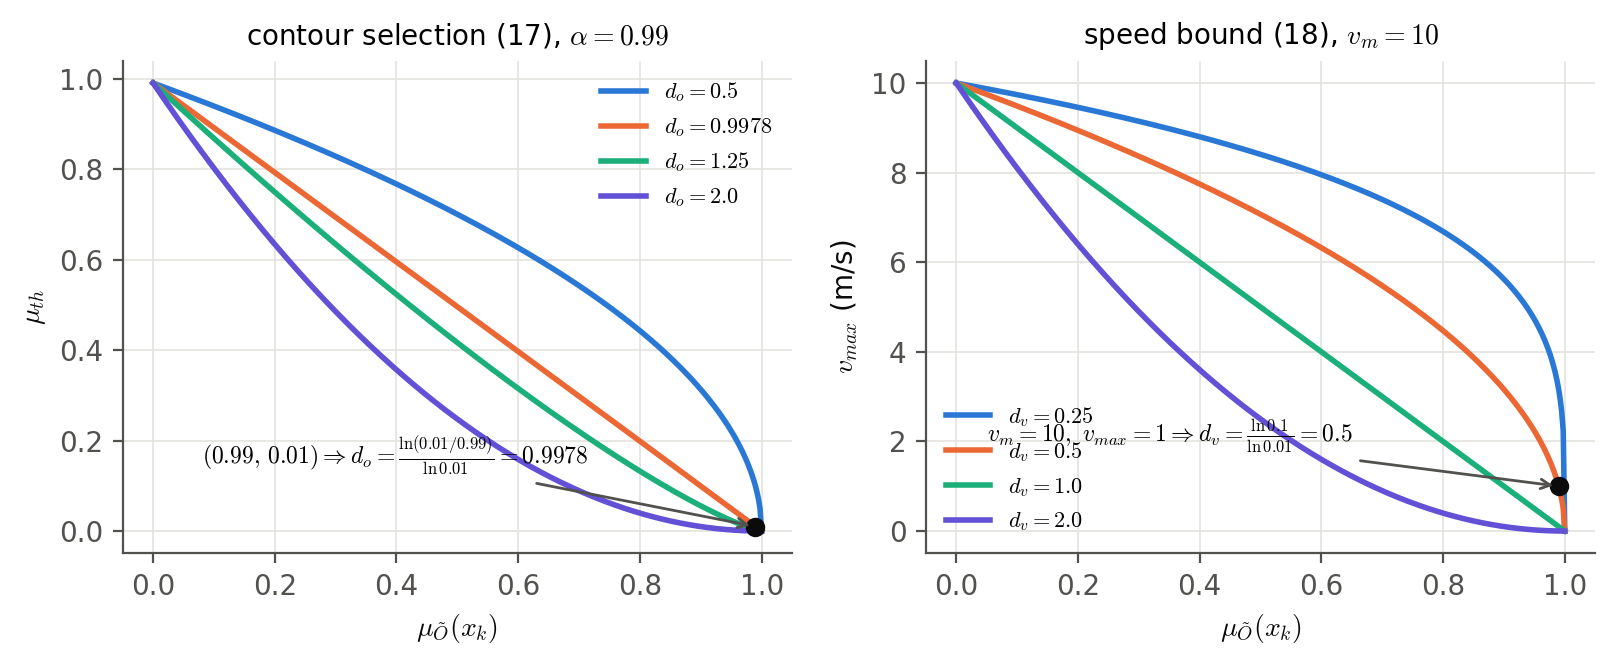
\includegraphics[width=0.6\linewidth]{f08_tuning.png}
\end{frame}

\begin{frame}{The cost function}
Over each planning interval ($\mu_{th}$ and $v_{max}$ held fixed: zero-order hold):
\[
f^k(\x)=\tfrac12\big(\mu_{E^k}(\x)-\mu_{th}\big)^2+\int_{\bar C}\mu_{E^k}(\x)\,ds\tag{19}
\]
$\bar C$ is the arc of the level curve through $\x_k$, from $\x_k$ to the point closest to the target. On $\bar C$ the integrand is constant, equal to $\mu_{E^k}(\x_k)$, so
\[
f^k(\x)=\tfrac12\big(\mu_{E^k}(\x)-\mu_{th}\big)^2+\mu_{E^k}(\x_k)\,\operatorname{length}(\bar C)\tag{20}
\]
\begin{itemize}
  \item Term 1 is minimised by moving \emph{across} level curves, along $\pm\nabla\mu_E$.
  \item Term 2 is minimised by moving \emph{along} the level curve towards the target.
  \item These directions are orthogonal, so the paper minimises the two terms independently.
\end{itemize}
\end{frame}

\begin{frame}{The update law}
Term 1 is handled by gradient descent. Term 2 has no closed form, but its descent direction is the unit tangent to the level curve:
\[
t(\x_k)=\pm R(\tfrac\pi2)\frac{\nabla\mu_{E^k}(\x_k)}{\|\nabla\mu_{E^k}(\x_k)\|_2},\qquad R(\tfrac\pi2)=\begin{bmatrix}0&-1\\1&0\end{bmatrix}\tag{21}
\]
\begin{block}{FPPA step (22)}
\[
\Delta\x_k=-\eta_n\big(\mu_{E^k}(\x_k)-\mu_{th}\big)\nabla\mu_{E^k}(\x_k)\;+\;\eta_t\,R(\tfrac\pi2)\frac{\nabla\mu_{E^k}(\x_k)}{\|\nabla\mu_{E^k}(\x_k)\|_2},\qquad \eta_t=v_{max}t_s
\]
\end{block}
\begin{columns}[T]
\column{0.45\textwidth}
\footnotesize
\textbf{Algorithm 1}
\begin{enumerate}\setlength\itemsep{0pt}
\item detect objects; cover them with atoms
\item atomic obstacles (2), (3), (6); union (4), (5)
\item fuzzy waypoints (8)--(10); fuzzy path (11), (12)
\item environment episode (15), (16)
\item apply (17), (18), (22); repeat every $t_s$
\end{enumerate}
\column{0.55\textwidth}
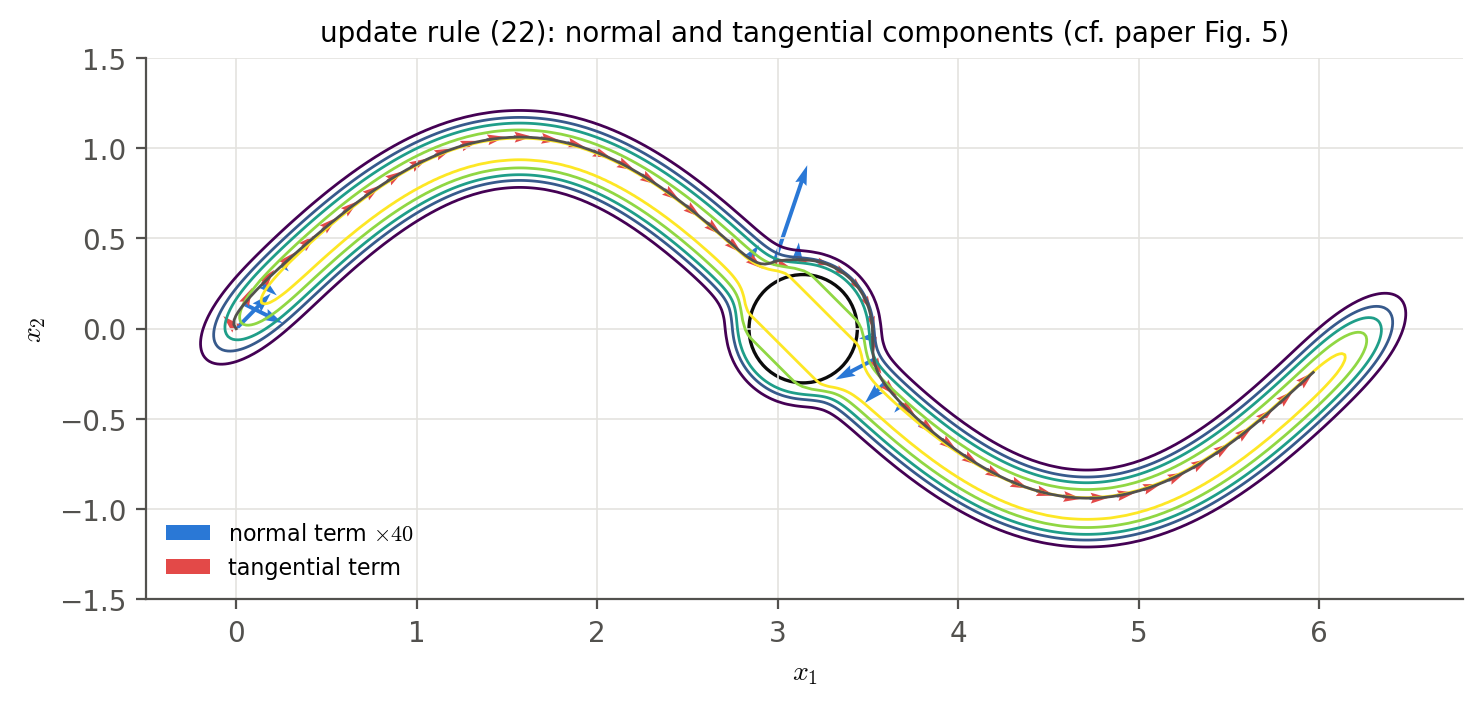
\includegraphics[width=0.88\linewidth]{f06_update_rule.png}
\end{columns}
\end{frame}

% ===========================================================================
\section{Our analysis}
% ===========================================================================
\begin{frame}{Why the law tracks a level curve: a Lyapunov argument}
Consider the continuous-time limit ($\mu:=\mu_{E^k}$, set-point $c(t)=\mu_{th}$, speed $v>0$) on $\{\nabla\mu\neq0\}$:
\[
\dot\x=-\eta_n(\mu(\x)-c)\nabla\mu(\x)+v\,R(\tfrac\pi2)\frac{\nabla\mu(\x)}{\|\nabla\mu(\x)\|}.
\]
\begin{proposition}[Our analysis]
Let $V(\x,t)=\tfrac12(\mu(\x)-c(t))^2$. Then
\[
\dot V=-\eta_n(\mu-c)^2\|\nabla\mu\|^2\;-\;(\mu-c)\,\dot c .
\]
\begin{enumerate}
  \item For constant $c$, $V$ is non-increasing and the tangential term does not affect it.
  \item The speed along the level curve is exactly $v$, so $\operatorname{length}(\bar C)$ decreases at rate $v$.
  \item If $c$ is constant, $\{\mu\ge\mu(\x_0)\}$ is compact, and $\nabla\mu\neq0$ there, then LaSalle's principle gives $\mu(\x(t))\to c$.
\end{enumerate}
\end{proposition}
\emph{Proof.} $\dot V=(\mu-c)(\nabla\mu^T\dot\x-\dot c)$ and $\nabla\mu^TR(\frac\pi2)\nabla\mu=0$, since $R(\frac\pi2)$ is skew-symmetric. \qed
\end{frame}

\begin{frame}{Numerical check of the proposition (Example 3)}
\centering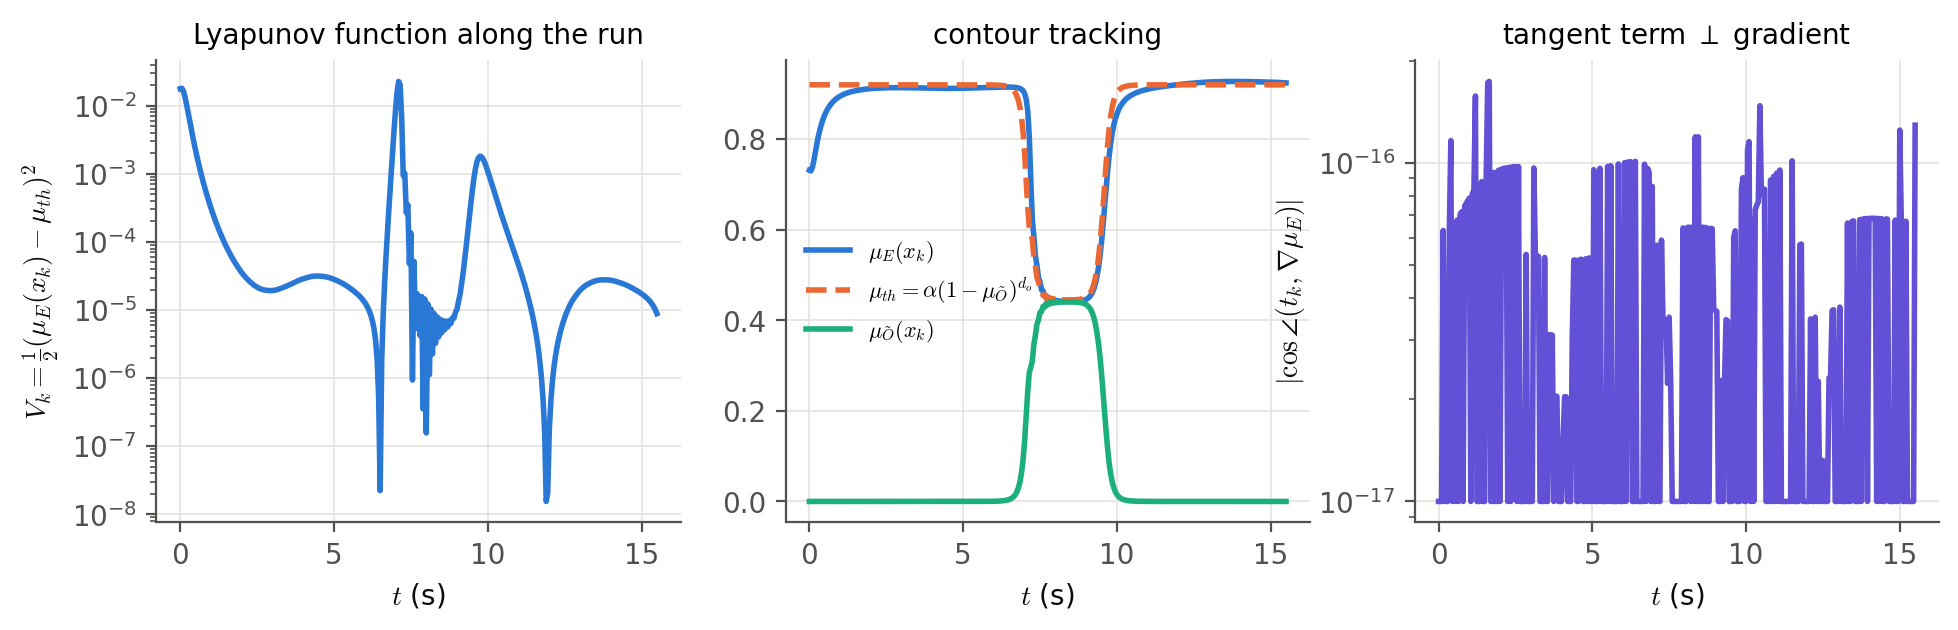
\includegraphics[width=\linewidth]{f07_lyapunov.png}
\begin{itemize}\small
  \item $V_k$ decays while $\mu_{th}$ is constant ($t<6$\,s, $t>10$\,s). It rises at $t\approx7$\,s and $t\approx10$\,s, exactly when $\dot c\ne0$, as predicted by the $-(\mu-c)\dot c$ term.
  \item The small residual oscillation comes from discretisation: a straight tangential step of length $\eta_t$ leaves a curved level curve by $\mathcal O(\kappa\,\eta_t^2)$, where $\kappa$ is the curvature.
  \item $|\cos\angle(t_k,\nabla\mu_E)|\le 2\times10^{-16}$: the tangent term is orthogonal to the gradient to machine precision.
\end{itemize}
\end{frame}

\begin{frame}{Orientation lemma: why obstacles are always passed on one side}
\begin{proposition}[Our analysis]
With the $+$ sign in (21), the super-level set $\{\mu_E>\mu_{th}\}$ always lies to the \emph{right} of the direction of motion.
\end{proposition}
\emph{Proof.} The motion direction is $t=R(\frac\pi2)\nabla\mu/\|\nabla\mu\|$, so $\nabla\mu/\|\nabla\mu\|=R(-\frac\pi2)\,t$, which is $t$ turned clockwise, i.e.\ to the right. $\mu$ increases in the direction of $\nabla\mu$. \qed

\medskip
\textbf{Consequences}
\begin{itemize}
  \item Path core and obstacles both belong to the super-level set, so the vehicle runs \emph{left} of the path and keeps every obstacle on its right. This is the paper's ``bypass from the left'' and ``clockwise'' choice.
  \item \alert{Level curves are closed.} At the end of the path the tracked curve turns back, so a stopping rule is required (we stop when the projection onto the path is within 1.5 segments of the end).
  \item If $\mu_{th}$ is so high that the vehicle sits on the \emph{ridge} of $\mu_P$, then $\nabla\mu$ flips sign across the ridge, and so does the direction of travel (next slides).
\end{itemize}
\end{frame}

\begin{frame}{How high is the fuzzy path? A Poisson-summation computation}
Take a straight path, uniform spacing $\Delta$, and $\Gamma_j=\operatorname{diag}(\gamma\Delta,\sigma)$. A point at lateral offset $y$ and longitudinal phase $\tau\in[0,1)$ gives
\[
\Sigma(y,\tau):=\sum_j\mu_{W_j}=e^{-y^2/2\sigma^2}\sum_{k\in\mathbb Z}e^{-(k+\tau)^2/2\gamma^2}.
\]
\begin{proposition}[Our analysis]
\[
\sum_{k\in\mathbb Z}e^{-(k+\tau)^2/2\gamma^2}=\gamma\sqrt{2\pi}\Big(1+2\sum_{n\ge1}e^{-2\pi^2\gamma^2n^2}\cos2\pi n\tau\Big).
\]
For $\gamma=0.75$: $\Sigma(0,\cdot)=1.8800$ with relative ripple $2e^{-2\pi^2\gamma^2}=3\times10^{-5}$, independent of $\Delta$.
\end{proposition}
\emph{Proof.} Poisson summation $\sum_k f(k+\tau)=\sum_n\hat f(n)e^{2\pi in\tau}$ with $f(x)=e^{-x^2/2\gamma^2}$, $\hat f(\xi)=\gamma\sqrt{2\pi}e^{-2\pi^2\gamma^2\xi^2}$. \qed
\begin{itemize}
  \item The fuzzy path is a ``Gaussian tube'' $\mu_P(y)\approx\sat\!\big(\gamma\sqrt{2\pi}\,e^{-y^2/2\sigma^2}\big)$.
  \item The longitudinal ripple is negligible, so on the ridge $\nabla\mu_P\approx0$ and the tangent (21) is ill-conditioned.
\end{itemize}
\end{frame}

\begin{frame}{Corollary: feasibility of $\alpha$, and a closed-form offset}
\begin{columns}[T]
\column{0.5\textwidth}
\begin{block}{Corollary (Our analysis)}
\begin{enumerate}
\item With the paper's $\tanh$: $\sup\mu_P=\tanh(\gamma\sqrt{2\pi})=\mathbf{0.9545}$ for $\gamma=0.75$. The set-point $\alpha=0.99$ is \alert{infeasible}. It is feasible iff
\[
\gamma>\gamma^*=\artanh(\alpha)/\sqrt{2\pi}=1.056 .
\]
\item With a range-preserving $\sat$, the vehicle settles at lateral offset
\[
y^*=\sigma\sqrt{2\ln\big(\gamma\sqrt{2\pi}/\alpha\big)} .
\]
\end{enumerate}
\end{block}
\small Case study 1 ($\sigma=1$, $\gamma=0.75$, $\alpha=0.99$): theory $y^*=\mathbf{1.1325}$\,m, simulation $\mathbf{1.1341}$\,m.
\column{0.5\textwidth}
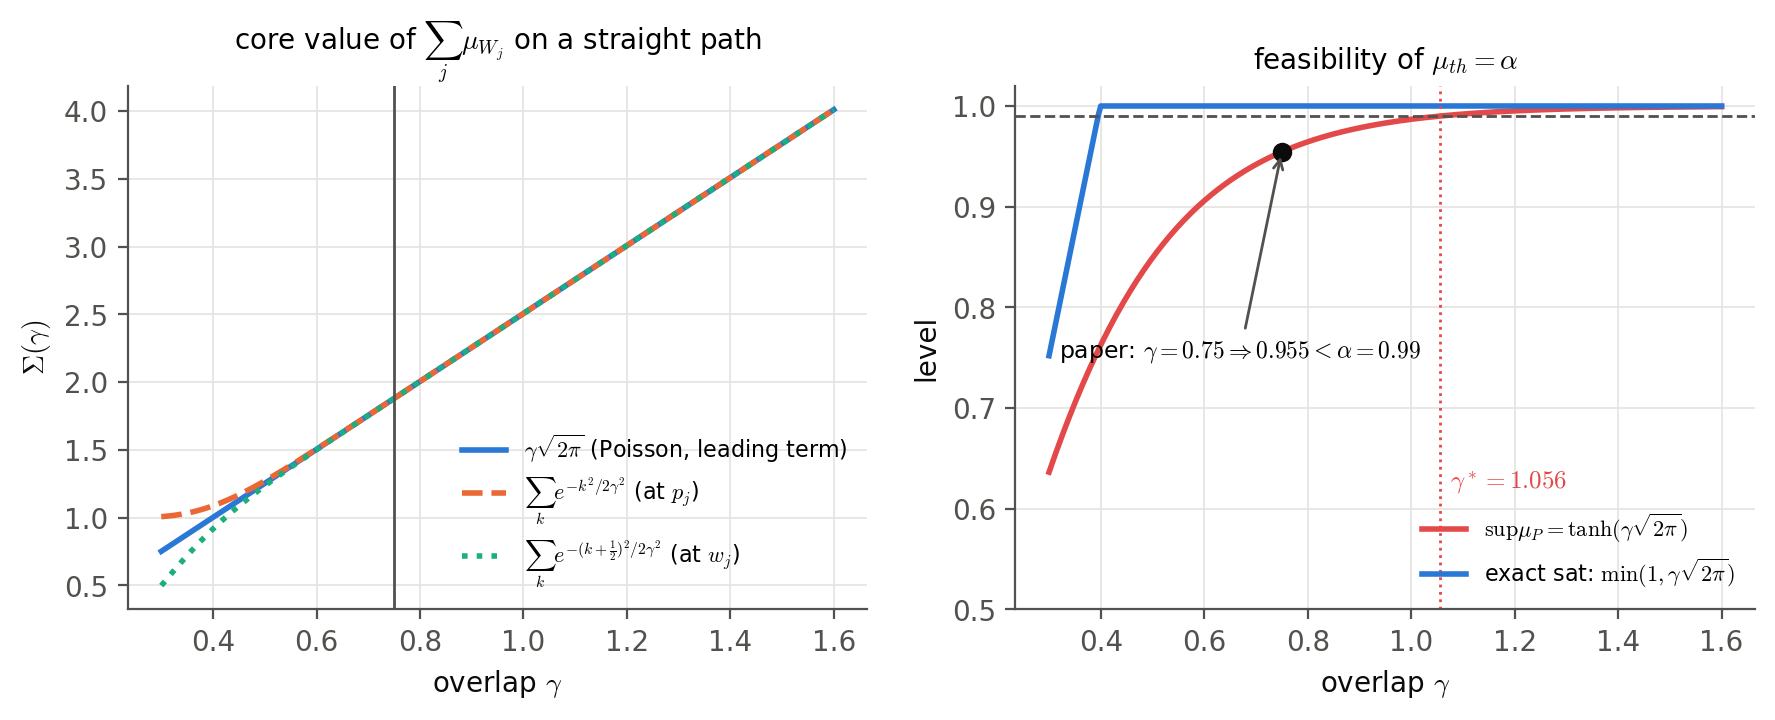
\includegraphics[width=\linewidth]{f09_core_level.png}

\small If $\alpha>\sup\mu_E$ then $V\ge\frac12(\alpha-\sup\mu_E)^2>0$ for all time. By the Lyapunov proposition the flow is driven to the ridge $\{\partial_y\mu=0\}$, where $t(\x)$ is discontinuous.
\end{columns}
\end{frame}

\begin{frame}{The infeasible set-point in practice}
\centering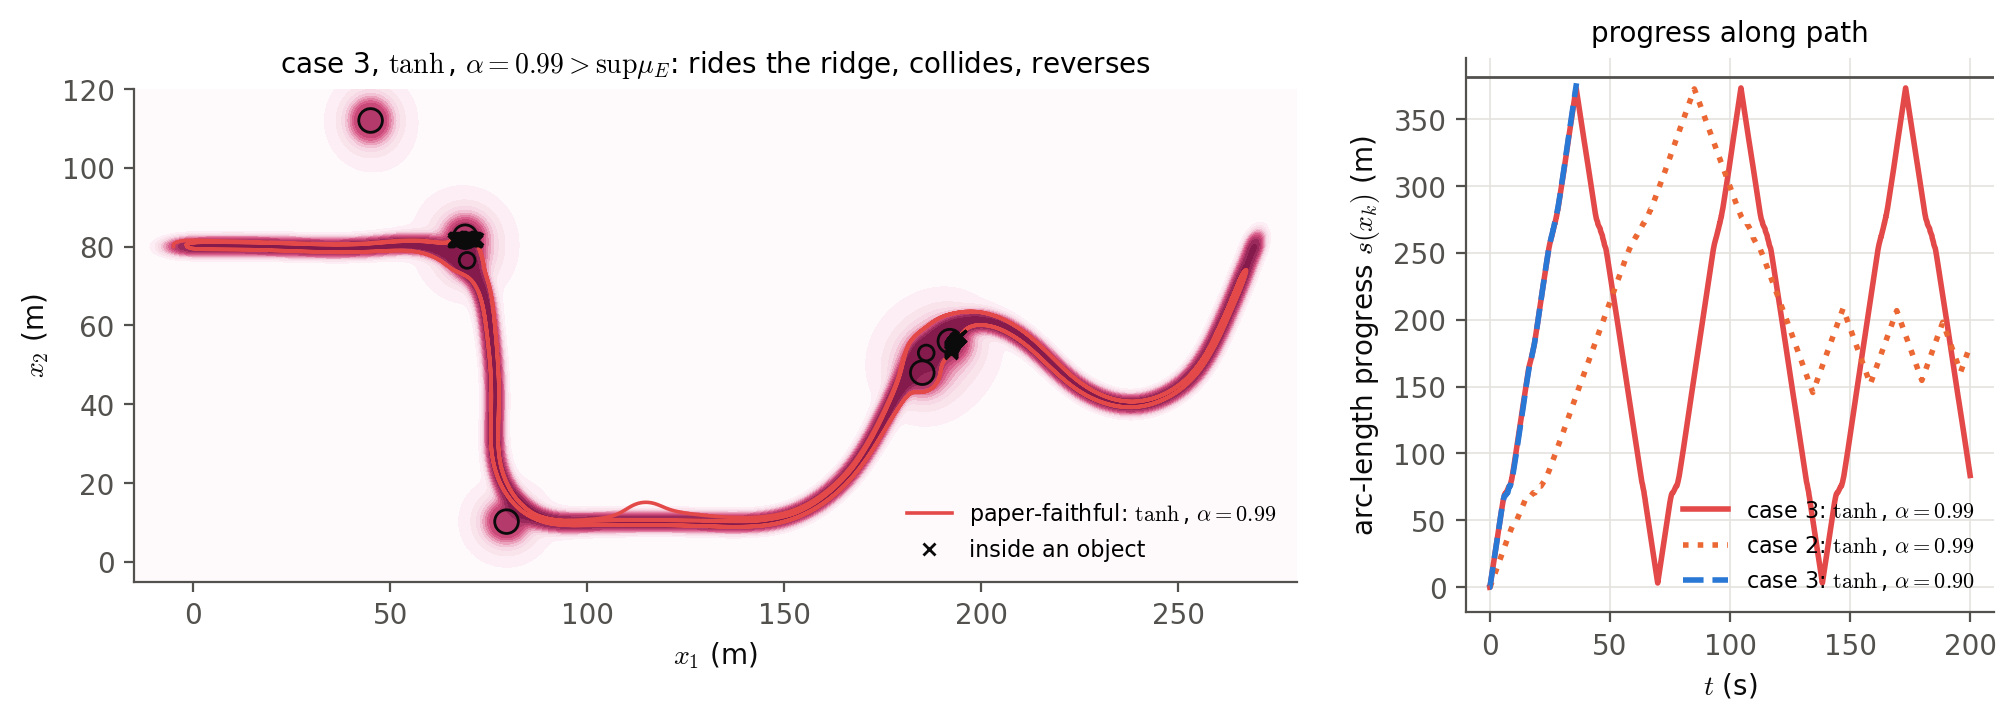
\includegraphics[width=0.82\linewidth]{f14_tanh_failure.png}
\begin{itemize}\small
  \item Paper-faithful ($\tanh$, $\alpha=0.99$), case 3 ($v_m=12$\,m/s): the vehicle rides the ridge, \alert{enters $O_2$ at $t=6.4$\,s} and later $O_4$, then turns around at the end of the path and travels it backwards. Case 2 also turns back about 9\,m short of the goal.
  \item The same planner with a feasible $\alpha=0.90<0.9545$, or with the softmin saturation and $\alpha=0.99$, completes every scenario.
  \item The paper reports success with $\alpha=0.99$. Its implementation details (bracketing of unions, saturation) must therefore differ from what the text states.
\end{itemize}
\end{frame}

% ===========================================================================
\section{Simulations}
% ===========================================================================
\begin{frame}{Simulation setup (Python / NumPy re-implementation)}
\begin{columns}[T]
\column{0.5\textwidth}
\textbf{Vehicle:} unicycle
\[
\dot x_1=v\cos\psi,\quad \dot x_2=v\sin\psi,\quad\dot\psi=\omega,\tag{23}
\]
with $v,\psi,\omega$ recovered by differentiating the planned positions, as in the paper. $t_s=50$\,ms, $p=1$, $r_i=1.25$\,m.

\medskip
\textbf{Parameters (paper):} $b=1.25$, $\alpha=0.99$, $\delta=0.1$, $d_v=0.5$, $d_o=1.25$, $\eta_n=0.75$, $\eta_t=v_{max}t_s$, $\gamma=0.75$.
\column{0.48\textwidth}
\textbf{Scenarios}
\begin{itemize}\small
\item Case 1: straight path, 100 waypoints, $\sigma=1$; concave arc of radius 30\,m, 97 atoms ($\lambda_i=0.25$).
\item Case 2: curved path, waypoints $\ge5$\,m apart, $\sigma=1.5$; 7 objects (Table 1), 2 of them moving. $v_m=5$\,m/s.
\item Case 3: as case 2 with $v_m=12$\,m/s.
\end{itemize}
\textbf{Assumptions} (not given in the paper)
\begin{itemize}\small
\item case 2 path digitised from Fig.~11;
\item velocity directions: $O_6\downarrow$, $O_7\rightarrow$;
\item baseline: a generic path-guided APF (\emph{not} the exact IAPF of ref.~[37]).
\end{itemize}
\end{columns}
\end{frame}

\begin{frame}{Case study 1: a concave obstacle}
\centering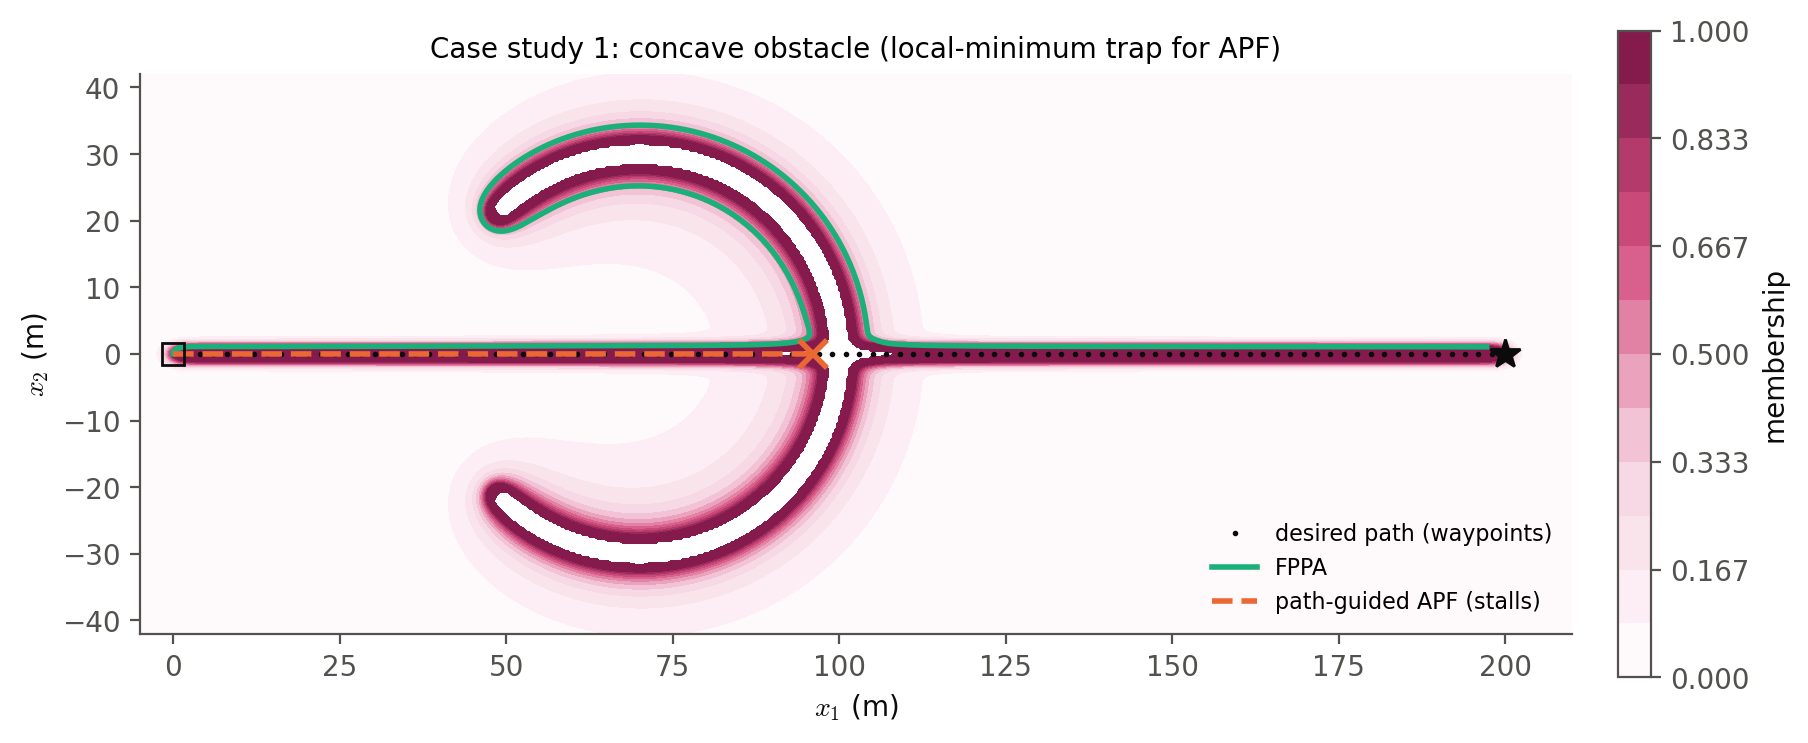
\includegraphics[width=0.78\linewidth]{f10_case1_path.png}
\begin{itemize}\small
\item The \textbf{APF stalls} inside the cup at $(96.1,0)$: attraction and repulsion balance (a local minimum).
\item The \textbf{FPPA} follows the level curve around the whole upper arm and back to the path. It finishes in $78.1$\,s (paper: $\approx78$\,s) with minimum clearance $2.37$\,m. The paper's Fig.~6 shows the same shape.
\item Why there is no trap: the tangent term has norm $\eta_t>0$ wherever $\nabla\mu_E\ne0$, so the method stops only at critical points of $\mu_E$.
\end{itemize}
\end{frame}

\begin{frame}{Case study 1: kinematic signals}
\centering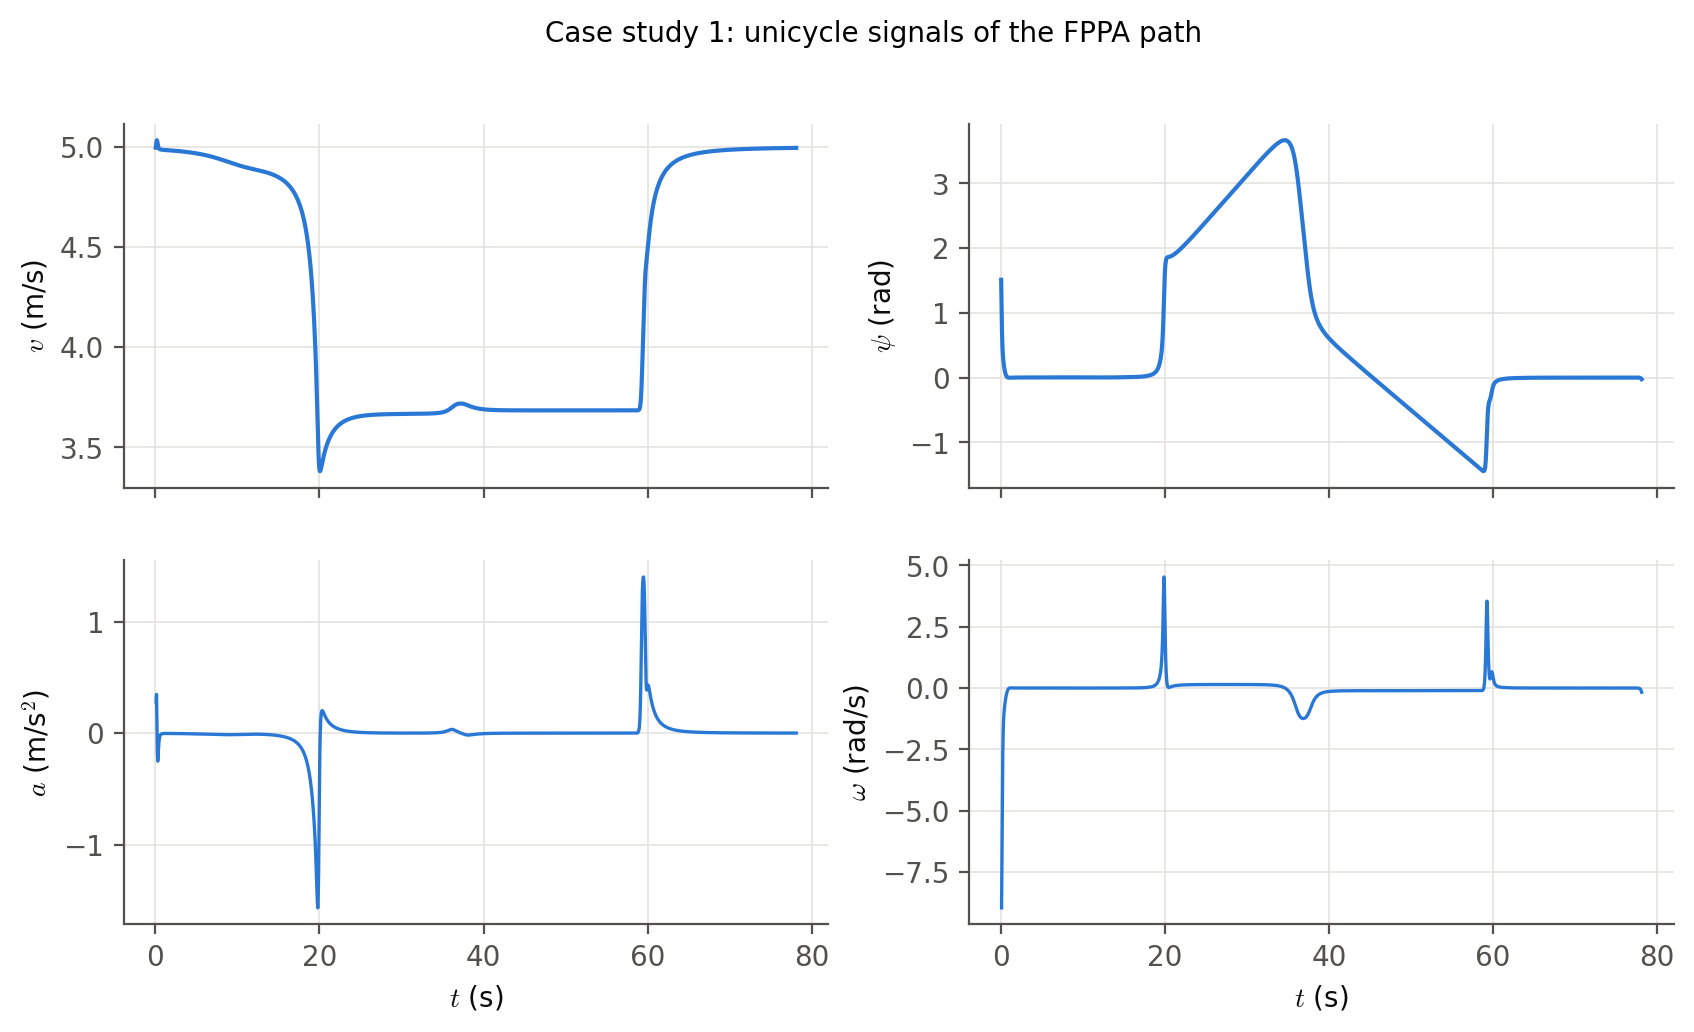
\includegraphics[width=0.7\linewidth]{f11_case1_signals.png}

\small The speed drops to $\approx3.3$\,m/s near the arc, as dictated by (18). The heading winds by about $+3.6$ rad around the arm, as in the paper's Fig.~8. Spikes in $\omega$ occur where the tracked level curve has high curvature (the arm tips).
\end{frame}

\begin{frame}{Case study 2: static and moving obstacles, $v_m=5$\,m/s}
\centering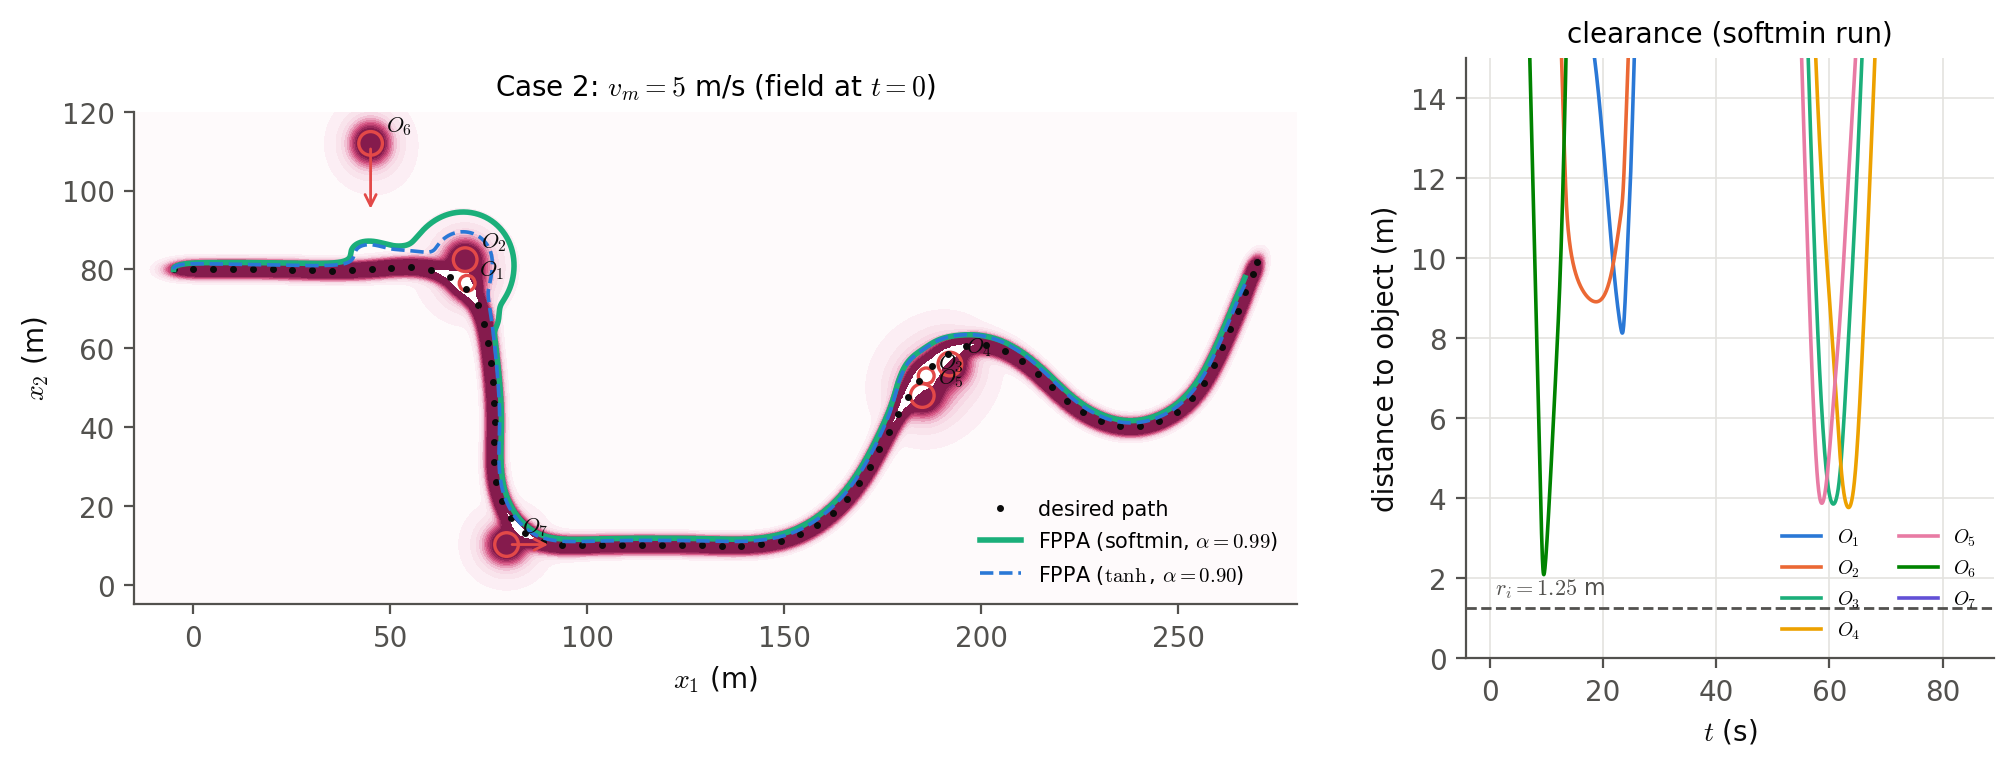
\includegraphics[width=\linewidth]{f12_case2_path.png}
\begin{itemize}\small
\item It completes in $84.8$\,s. Minimum clearance is $2.09$\,m (moving $O_6$); every object stays above $r_i=1.25$\,m.
\item Around $O_1,O_2$ the vehicle takes a wide detour above the pair, as in the paper's Fig.~11: the bypass side is fixed by the orientation lemma, not chosen for path length.
\end{itemize}
\end{frame}

\begin{frame}{Case study 2: kinematic signals}
\centering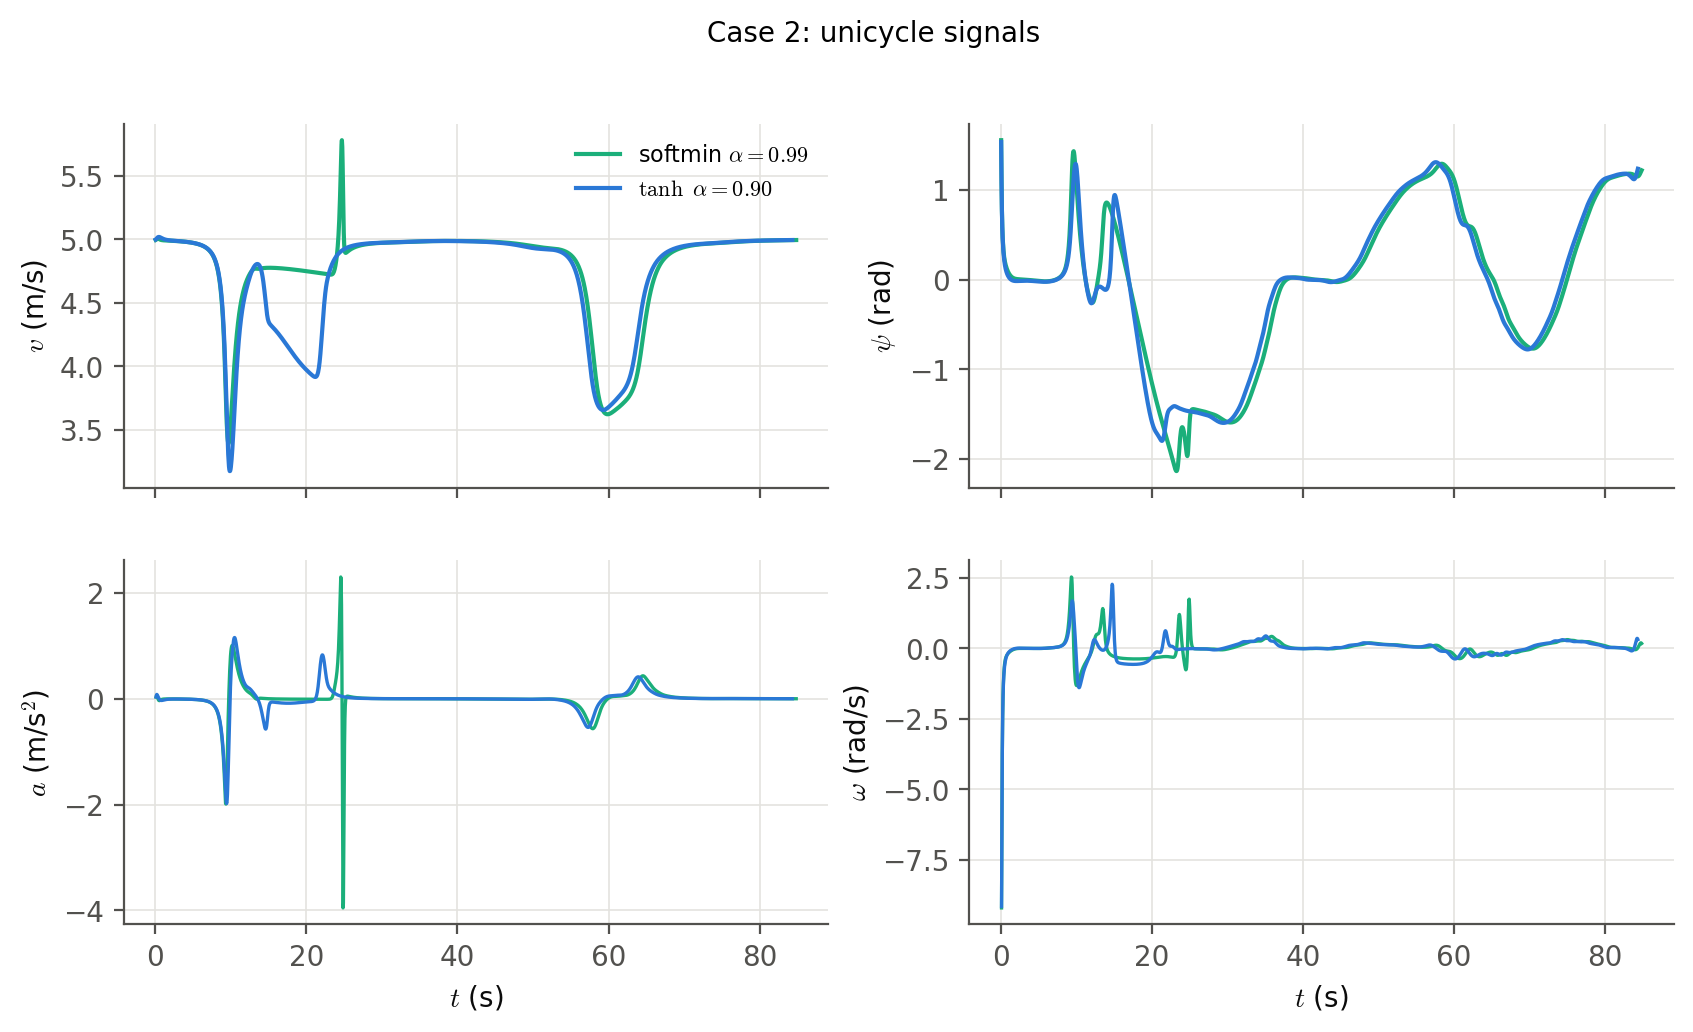
\includegraphics[width=0.7\linewidth]{f13_case2_signals.png}

\small Smooth speed and heading profiles; $|a|\le4.0$\,m/s$^2$ and $|\omega|\le9.2$\,rad/s.
\end{frame}

\begin{frame}{Case study 3: high speed, $v_m=12$\,m/s}
\centering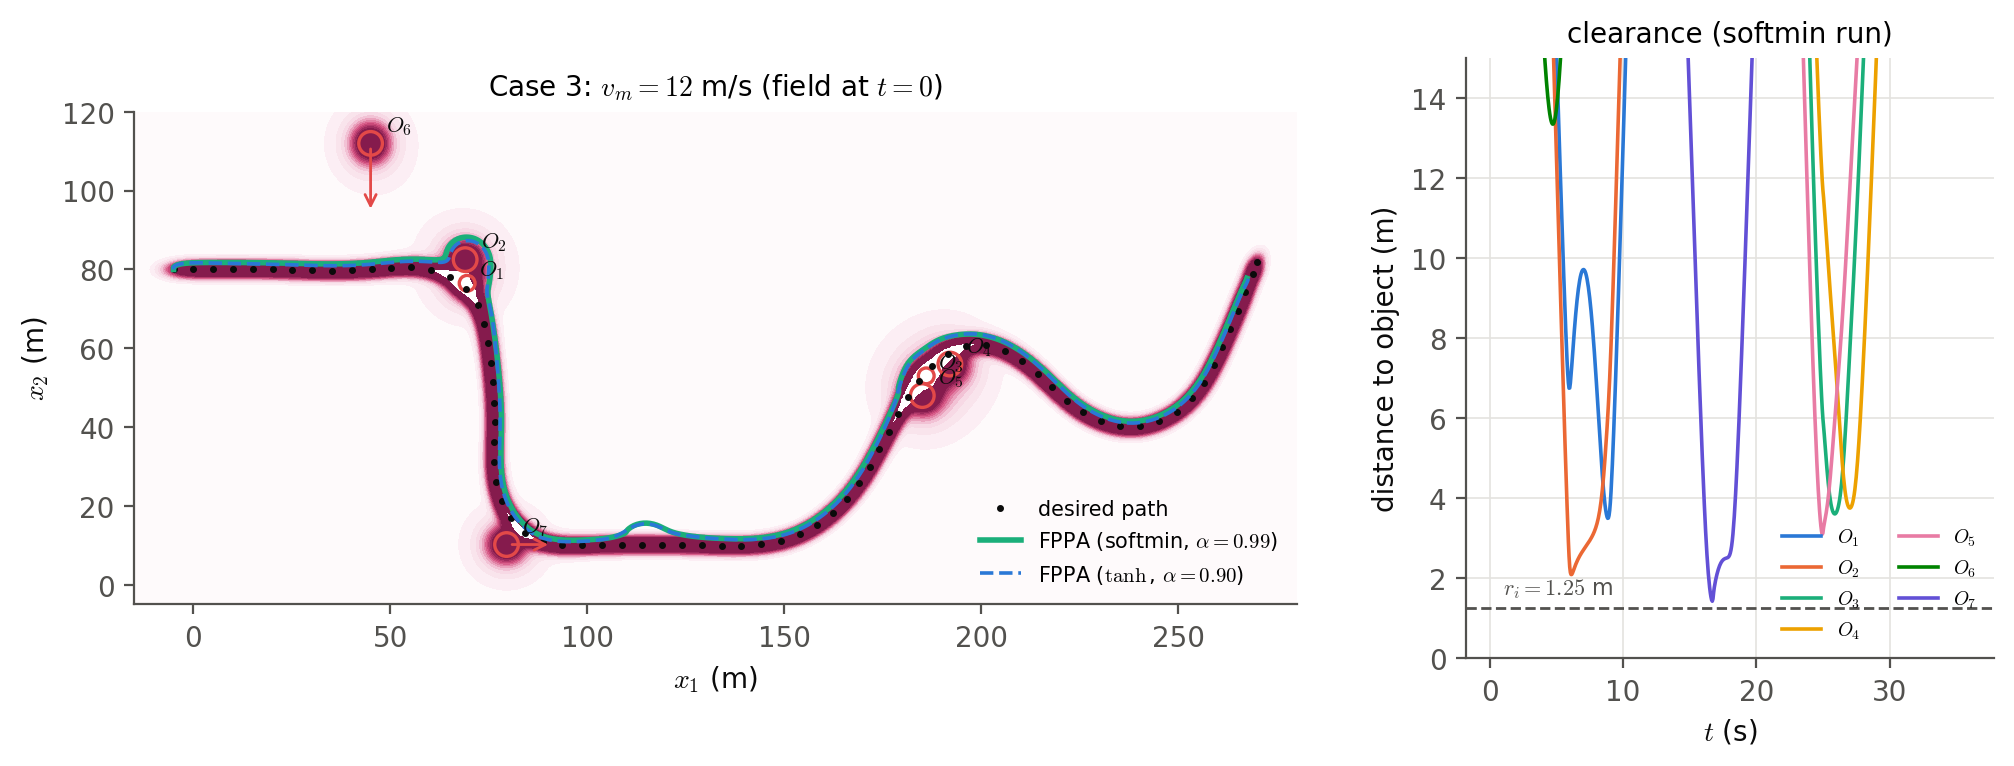
\includegraphics[width=\linewidth]{f12_case3_path.png}

\vspace{-1ex}
\begin{itemize}\small
\item With softmin it completes in $36.1$\,s with minimum clearance $1.43$\,m ($O_7$, overtaken from the left). No re-tuning was needed, as the paper claims.
\item $\tanh$ with $\alpha=0.90$ also completes, but passes $O_2$ at $1.03$\,m, inside the $1.25$\,m safety margin.
\end{itemize}
\end{frame}

\begin{frame}{Case study 3: kinematic signals}
\centering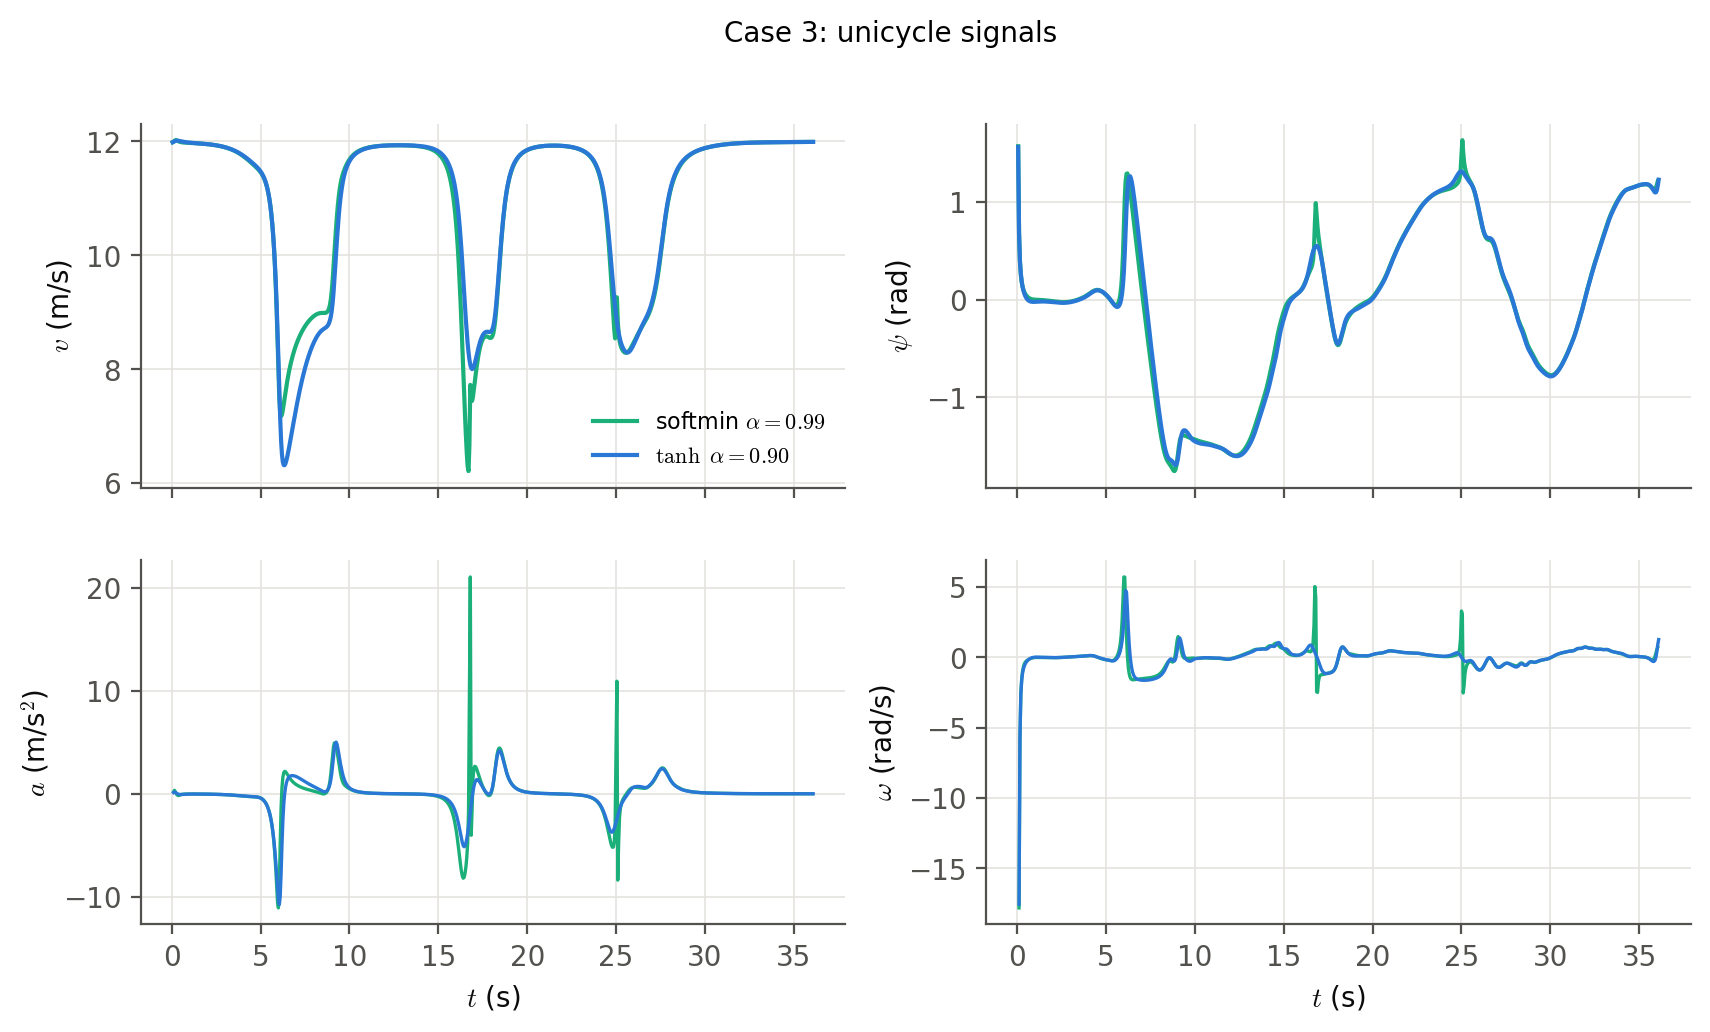
\includegraphics[width=0.7\linewidth]{f13_case3_signals.png}

\small At 12\,m/s single-step spikes appear in $a$ (up to $21$\,m/s$^2$) where $\mu_{th}$ jumps between intervals (zero-order hold). This is the discrete counterpart of the $-(\mu-c)\dot c$ term; a rate limit on $\mu_{th}$ would remove it.
\end{frame}

\begin{frame}{Summary of results}
\centering\small
\begin{tabular}{@{}llrrrl@{}}
\toprule
Scenario & Variant & Time [s] & min.\ clearance [m] & $\max|a|$ & Outcome\\
\midrule
Case 1 & softmin, $\alpha=0.99$ & 78.1 & 2.37 & 1.6 & \checkmark\\
       & $\tanh$, $\alpha=0.99$ (paper) & 78.3 & 2.27 & 1.6 & \checkmark\ (rides the ridge)\\
       & APF baseline           & ---  & ---  & --- & stalls at $(96.1,0)$\\
Case 2 & softmin, $\alpha=0.99$ & 84.8 & 2.09 & 4.0 & \checkmark\\
       & $\tanh$, $\alpha=0.90$ & 84.3 & 1.31 & 2.0 & \checkmark\\
       & $\tanh$, $\alpha=0.99$ (paper) & --- & 0.21 & --- & turns back, oscillates\\
Case 3 & softmin, $\alpha=0.99$ & 36.1 & 1.43 & 21.1 & \checkmark\\
       & $\tanh$, $\alpha=0.90$ & 36.1 & 1.03 & 10.8 & \checkmark\ (margin violated)\\
       & $\tanh$, $\alpha=0.99$ (paper) & --- & $<0$ & --- & \alert{collision} ($O_2$, $O_4$)\\
\bottomrule
\end{tabular}

\medskip
\begin{columns}[c]
\column{0.4\textwidth}
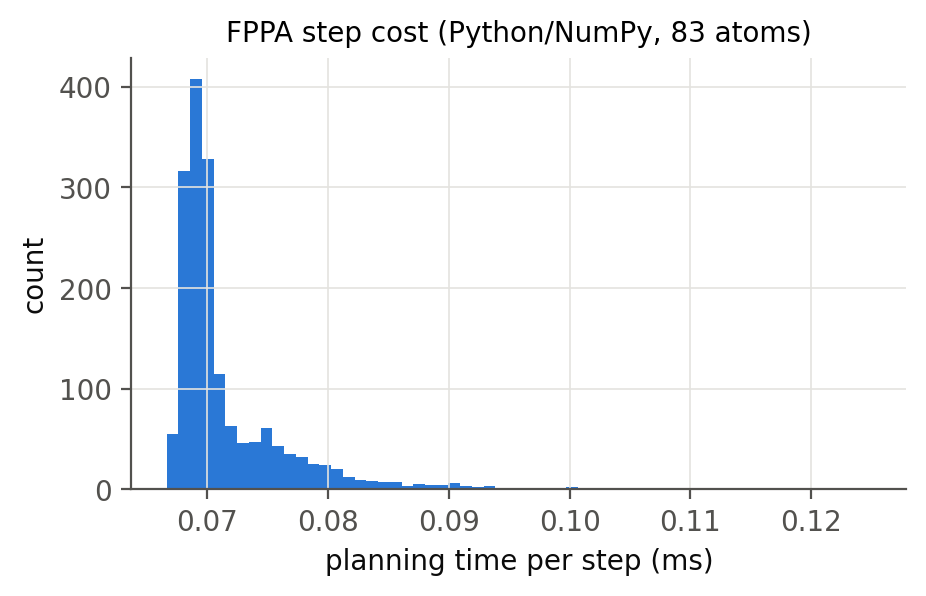
\includegraphics[width=0.8\linewidth]{f15_cpu.png}
\column{0.5\textwidth}
\small\textbf{Cost:} a planning step evaluates one closed-form $\mu_E$ and its gradient, $\mathcal O(N+M)$ atoms. Median $0.07$\,ms in NumPy (84 atoms; paper: $<0.3$\,ms in MATLAB), versus $t_s=50$\,ms, so it runs in real time.
\end{columns}
\end{frame}

% ===========================================================================
\section{Assessment}
% ===========================================================================
\begin{frame}{Critical assessment}
\begin{columns}[T]
\column{0.5\textwidth}
\textbf{Strengths}
\begin{itemize}\small
\item A single algebraic object $\mu_E$ encodes the path, the obstacles and the perception uncertainty.
\item Yager's union gives an $\mathcal O(N)$ closed form with tunable conservativeness ($p$).
\item No APF-type local minima: motion is along level curves, not down a potential.
\item Smooth, real-time, and transfers across speeds.
\end{itemize}
\column{0.5\textwidth}
\textbf{Mathematical gaps we found}
\begin{itemize}\small
\item $\tanh$ smoothing breaks the t-conorm axioms and associativity (Prop.~\ref{prop:tanh}).
\item The set-point $\alpha=0.99$ is infeasible for $\gamma=0.75$ (Poisson corollary).
\item $t(\x)$ is undefined at critical points of $\mu_E$ (ridges, saddles between obstacles).
\item Level curves are closed, so a stopping rule is needed.
\item No formal collision-avoidance guarantee: it depends on $d_o,\eta_n$ versus speed.
\item Notation: (10) should read $H D H^T$; Def.~1 core; $p\to0^+$ vs.\ drastic sum.
\end{itemize}
\end{columns}
\end{frame}

\begin{frame}{Conclusions}
\begin{itemize}
  \item We re-implemented every equation of the paper, with exact gradients, and reproduced Examples 1--3 and the three case studies.
  \item The fuzzy-set picture is sound: the planner is a level-curve follower on a Yager union of convex fuzzy atoms. A Lyapunov function explains why it tracks $\{\mu_E=\mu_{th}\}$, and an orientation lemma explains the ``always pass on the left'' behaviour.
  \item Poisson summation gives the height of the fuzzy path in closed form, $\sup\mu_P=\sat(\gamma\sqrt{2\pi})$. This yields a feasibility condition on $\alpha$ and the lateral offset $y^*$, matched by simulation to $2$\,mm.
  \item With a range-preserving smooth saturation (or a feasible $\alpha$), the method avoids the concave-obstacle trap and handles moving obstacles at 5 and 12\,m/s.
\end{itemize}
\vfill
\small Code: \texttt{fppa/} (model and planner), \texttt{experiments/} (all figures, \texttt{results.json}); animation \texttt{figures/case2\_animation.gif}.
\end{frame}

\appendix
\begin{frame}{Appendix: all gradients used}
\small
\begin{align*}
\text{obstacle atom:}\quad & \nabla_\x\mu_{\Ot_i}= -2b\,\operatorname{sech}^2(s_i^{-b})\,s_i^{-b-1}\,\Lambda_i^{-1}\chi_i,\qquad \chi_i=\Lambda_i^{-1}(\x-\cc_i),\ s_i=\chi_i^T\chi_i\\
\text{waypoint:}\quad & \nabla_\x\mu_{W_j}=-\mu_{W_j}(\x)\,\Gamma_j^{-2}(\x-\pp_j)\\
\text{union:}\quad & \nabla\big(\sat_\bullet(\|\mathbf a(\x)\|_p)\big)=\sat_\bullet'(n)\sum_i (a_i/n)^{p-1}\nabla a_i,\qquad n=\|\mathbf a\|_p\\
& \tanh'(n)=1-\tanh^2 n,\qquad \sat_\kappa'(n)=1-\big(1+e^{-\kappa(n-1)}\big)^{-1}\\
\text{FPPA step:}\quad & \Delta\x_k=-\eta_n(\mu_E-\mu_{th})\nabla\mu_E+v_{max}t_s\,R(\tfrac\pi2)\nabla\mu_E/\|\nabla\mu_E\|
\end{align*}
\textbf{Numerical safeguards:} $s\ge10^{-9}$; $\operatorname{sech}^2$ computed as $1-\tanh^2$, which gives exactly $0$ once $\tanh$ saturates; $\|\cdot\|_p$ computed with max-scaling, as in \texttt{hypot}, to avoid underflow of $a^p$.
\end{frame}

\end{document}
